\documentclass[11pt,a4paper]{report}

\usepackage[polish]{babel}
\usepackage[utf8x]{inputenc}
\usepackage{polski}
%\usepackage[T1]{fontenc}
\frenchspacing

\usepackage{multirow}
\usepackage{indentfirst}
\usepackage{amsthm}
\usepackage{amsmath}
\usepackage{algorithmic}
\usepackage{algorithm}
\usepackage{array}
\usepackage{graphicx}
\usepackage{listings}
\usepackage{listing}
\usepackage{float}
\usepackage{colortbl}


\newtheorem{definicja}{Definicja}
\newtheorem{Observ}{Obserwacja}
\definecolor{kugray5}{RGB}{224,224,224}

\pagenumbering{arabic}

\graphicspath{{img/}}

\begin{document}
\tableofcontents
%\input{wstep}

\chapter{Opis problemu}

Praca ma na celu zbadanie problemu wyliczania rankingu dokumentów w sieciach społecznościowych w czasie wyszukiwania wyników zapytania. Badanie w tej pracy sieci społecznościowe charakteryzują się tym,że zasoby przechowywane przez nie zostały przez różnych użytkowników wybranymi etykietami (zwanymi również annotacjami czy tagami). Jako dodatkowy element, w czasie wyszukiwania dokumentów zostaną użyte dane mówiące o popularności danych wyników, pozyskane z rożnych serwisów społecznościowych, takich jak twitter, facebook czy digg. Dane te powinny polepszyć jakoś wyszukiwania i przyśpieszyć obliczenia potrzebne do wyliczenia statycznych rankingów dokumentów. 
%\documentclass[11pt,a4paper]{report}

%\usepackage[polish]{babel}
%\usepackage[utf8x]{inputenc}
%\usepackage{polski}



%\frenchspacing
%\usepackage{indentfirst}
%\usepackage{amsthm}
%\usepackage{amsmath}
%\usepackage{algorithmic}
%\usepackage{algorithm}
%\usepackage{array}
%\usepackage{multirow}
%\usepackage{graphicx}
%\usepackage{listings}
%\usepackage{float}
%\pagenumbering{arabic}

%\graphicspath{{img/}}

%\begin{document}
%\tableofcontents
\chapter{Wprowadzenie}

\section{Opis problemu}
Obecnie prowadzonych jest wiele badań nad sieciami społecznymi używającymi etykiet (tzw. tagów, czy adnotacji) do porządkowania zasobów użytkownika. Część z nich za cel stawia sobie ulepszenie algorytmów wyszukiwania dokumentów, inne używają tych zasobów dla personalizacji wyników dla użytkowników, rekomendacji dokumentów, użytkowników, czy tagów w czasie procesu etykietowania.

Autorzy prac \cite{yanbe2007} i \cite{citeulike:3423869} analizują użyteczność etykietowania dokumentów przy wyszukiwaniu. Ich analizy bazują głównie na danych systemu delicious. Wnioski z tych prac są pozytywne. Zwracają one uwagę na korelacje miedzy popularnością stron w serwisie, a ich rankingiem według algorytmu PageRank. Dodatkowo wskazują na problemy z nowymi dokumentami dodanymi do sieci, z którymi mają problemy algorytmy bazujących na odnośnikach pomiędzy dokumentami, a które mogą być rozwiązane przez strony takie jak delicous. Również rozwiązanie problemu nowych danych jest zaproponowane w pracy \cite{citeulike:8024203}. W tym artykule, jako rozwiązania, autorzy proponują użycie informacji pobranych z systemu twitter, który służy do mikroblogowania. Pod uwagę brane są krótkie informacje umieszczane przez użytkowników zawierające odnośniki do dokumentów jak również inne informacje dostępne w ich profilach.


Autorzy pracy  zaprezentowali formalny model folksonomi. Folksonomią nazywamy społeczne klasyfikowanie czy tagowanie różnych zasobów. Formalnie model folksonomii został przedstawiony w pracy \cite{hotho2006information} i zdefiniowany został jako: 

\begin{definicja}
Folksonomia jest to krotka $F := (U,T,D,Y )$, gdzie:
\begin{itemize}
\item $U$,$T$ i $D$ są to zbiory skończone, których elementy nazywają się odpowiednio użytkownicy, tagi i dokumenty
\item $Y$ jest relacją między tymi elementami: $Y \subseteq  U \times T \times D $, nazywamy ją relacją przypisania tagu.

\end{itemize}
\end{definicja}


Również w  pracy \cite{hotho2006information} zaprezentowano algorytm AdaptedPageRank i jego bardziej spersonalizowana wersję algorytm FolkRank. Oba te algorytmy bazują na metodzie PageRank. Algorytm ten pozwala na rekomendacje tagów dla użytkowników jak również na ustalenie rankingu w wyszukiwanych elementach. Dokładny opis tych algorytmów znajduje się kolejnych rozdziałach.

W pracy \cite{bao2007social} przedstawione zostały algorytmy SocialSimRank i SocialPageRank. Algorytm SocialPageRank jest statycznym rankingiem zasobów, opartym również o ideę algorytmy PageRank. Algorytm ten bierze pod uwagę ilość tagów wskazujących na dany dokument jak również różną wagę opisujących dokument etykiet. Drugim proponowanym w tej pracy algorytmem jest SocialSimRank, który estymuje podobieństwo między używanymi tagami, a następnie wyniki te są używane dla wyliczanie podobieństwa między zapytaniem użytkownika a tagami przypisanymi do danego zasobu. Ten algorytm również zostanie dokładniej opisany w kolejnych rozdziałach.

W pracach \cite{citeulike:3063696} i \cite{citeulike:3423905} autorzy biorą pod uwagę całą sieć społecznościową użytkownika i wykorzystują te dane dla przedstawienia spersonalizowanych wyników. W artykule \cite{citeulike:3063696} opisywany jest algorytm ContextMerge, który wykonuje wyszukiwanie biorąc pod uwagę zależności między użytkownikami.  Dodatkowo pozwala na dynamiczne dodawanie nowych wyników do odpowiedzi dla uzyskania $k$. W pracy \cite{citeulike:3423905} autorzy zaproponowali system, który łączy wyniki wyszukiwarki z danymi użytkownikami aplikacji takich jak delicous. Jako bazowa wyszukiwarka może być użyta dowolna aplikacja, która zwraca dokumenty wraz z przypisanym do nich rankingiem. Wyniki te są następnie przeliczane za pomocą danych uzyskanych od użytkownika, czyli ze zbiorem dokumentów i tagów opisanych przez niego i innych użytkowników. Jako rezultat otrzymujemy nowy, bardziej spersonalizowany ranking dokumentów.

W pracy \cite{conf/mir/RawashdehKE11} celem autorów było spersonalizowanie wyników wyszukiwania w dokumentach z tagami. Do tego celu stworzone zostały dwa modele: użytkownik-tag, który ukazuje jak użytkownik użył tagi podobne do wybranego tagu. Drugim modelem jest model tag-zasób opisujący w jaki sposób dokumenty podobne do danego zasobu zostały opisane etykietami. 



Probabilistyczne podejście do rankingu dokumentów przy użyciu tagów zostało zaprezentowane w pracy \cite{citeulike:2775088} i \cite{citeulike:8846111}. W \cite{citeulike:2775088} autorzy zaprezentowali model probabilistyczny dla generowania etykiet i zależnych im dokumentów i wyszukiwania ich tematów. W \cite{citeulike:8846111} autorzy prezentują metodę rankingu tagów w zależności od ich tematu i konstruują graf przejścia między tagami należącymi do różnych tematów. Metoda ta jest wykorzystana następnie dla rekomendacji tagów dla użytkownika w czasie opisywania dokumentów. 







% [1] Web Search Personalization via Social Bookmarking and Tagging
% Michael G. Noll and Christoph Meinel
% http://data.semanticweb.org/pdfs/iswc-aswc/2007/ISWC2007_RT_Noll.pdf


% [2] can social bookmarkign enhance search in the web ?
%
% [3] can social bookmarking improve web search ?
%
% [4] time is of the essence: imprving recenct ranking using twitter data








% [7] exploring social annotations for information retrieval
% ding zhou

% [8] topic-based ranking in folksonomy via probabilistic model
% yan'an Jin

% [9] optimizing web search using social annotations

% [10] information retrieval in folksonomies: search and ranking

% [11] efficient top-k querying over Social-Tagging Networks

% [12] folksonomu-boosted social media search and ranking. 



% [5]  Exploring Folksonomy for Personalized Search  
%  http://datamining.dongguk.ac.kr/work/project/KDI/CVM/%EC%B5%9C%EC%A2%85%ED%99%94%EC%9D%BC-1.%EA%B2%BD%EB%82%A8%EB%A1%9C%EB%B4%87%EB%9E%9C%EB%93%9C%281%EC%B0%A8%EC%A1%B0%EC%82%AC%29/p155-xu-Exploring%20folksonomy%20for%20personalized%20search%20.pdf 


% [6] Personalization of Tagging Systems
% http://ict.ewi.tudelft.nl/pub/jun/ptIPM.pdf

% W mojej pracy skupie się na dwóch algorytmach: adapted pagerank i socialpagerank. Postaram się porownać wyniki działania tych dwóch algorytmów jak również zaproponuje użycie innych danych z innych serwisów społecznościowych takich jak twitter, facebook i digg do poprawienia jakości wyszukiwanych materiałów.






%\bibliographystyle{plain}
%\bibliography{biblio}


%\end{document}


\chapter{Algorytmy}


\section{Folksonomia}

Folksonomią nazywamy społeczne klasyfikowanie, czy tagowanie różnych zasobów. Formalnie model folksonomii został przedstawiony w pracy \cite{hotho2006information}. Można ja przedstawić jako krotkę $F := (U,T,R,Y)$, gdzie:
$U$,$T$,$R$ to zbiory skończone, których elementy składają się odpowiednio z użytkowników, tagów i dokumentów. $Y$ jest relacją “przypisania tagu” pomiędzy tymi elementami $Y \subseteq U \times T \times R$

Użytkownicy i tagi identyfikowani są na podstawie ich unikalnych nazw własnych. Dokumenty mogą być różnymi danymi: stronami www, zdjęciami, plikami np: pliki pdf. Ta praca bazuje na danych pobranych z witryny delicous, które w zdecydowanej większości są stronami www. Dane które nie są stroną www nie są brane pod uwagę w tej pracy. 





\chapter{SocialPageRank}
\section{Opis}
SocialPageRank jest algorytmem wyliczającym statyczny ranking stron z perspektywy użytkownika sieci. Algorytm bazuje na obserwacji relacji miedzy popularnymi stronami, tagami i aktywnymi użytkownikami. Popularne strony są dodawane przez aktywnych się użytkowników, które są opisywane popularnymi tagami. Aktywni się użytkownicy używają popularnych tagów dla popularnych stron. Popularne tagi używane są do annotacji popularnych stron przez ważnych użytkowników.

Bazując na powyższych założeniach algorytm propaguje i wzmacnia zależności między popularnymi tagami, użytkownikami i dokumentami. 
\subsection*{Dane wejsciowe:}
$N_T$: ilośc tagów

$N_U$: ilośc użytkowników

$N_D$: ilośc dokumentów

$M_{DU}$: macierz $N_D \times N_D$ asocjacyjna między dokumentami a użytkownikami

$M_{UT}$: macierz $N_U \times N_T$  asocjacyjna między użytkownikami a tagami

$M_{TD}$: macierz $N_T \times N_D$ asocjacyjna między tagami a dokumentami

$P_0$: wektor, o długości $N_D$, 

\subsection*{Inicjalizacja}
W komórce macierzy$M_{DU}(d_n, u_k)$ znajduje się wartość będąca ilością adnotacji przypisanych do dokumentu $d_n$ przez użytkownika $u_k$. Podobnie dla pozostałych macierzy, elementy $M_{UT}(u_k, t_n)$ to ilość dokumentów opisanych tagiem $t_n$ przez użytkownika $u_k$, elementy$M_{TD}(t_n, d_k)$: ile użytkowników dodawało dokument $d_k$ i oznaczyło go annotacją $t_n$. 

Wektor $P_0$ zainicializowany został losowymi wartościami z przedziału $[0,1]$. Jest on pierwszym przybliżeniem rank dokumentów.


\begin{algorithmic}
\REPEAT
\STATE $U_i = M_{DU}^T * P_i$
\STATE $T_i = M_{UT}^T * U_i$
\STATE $P_i’ = M_{TD}^T * T_i$
\STATE $T_i’ = M_{TD}  * P_i’$
\STATE $U_i’ = M_{UT} * T_i’$
\STATE $P_(i+1) = M_{DU} * U_i’$

\UNTIL{ wartości wektora $P_n$ nie zbiegną }
\end{algorithmic}

\subsection*{Złożność}
Złożoność czasowa każdej iteracji wynosi $O(N_u*N_d + N_t*N_d + N_t*N_u)$.

\section{Wyniki algorytmu dla przykładowych danych}

W poniższej tabelce znajdują sie dane, dla których zostało sprawdzone działanie algorytmu Social PageRank. Dane są nie duże i składają sie z trzech różnych dokumentów, dwóch użytkowników i trzech tagów.

\renewcommand{\multirowsetup}{\centering}
\begin{center}
\begin{tabular}{|l| r | r| }
\hline
\multirow{3}{5cm}{\centering Strony www}
& \multicolumn{2}{p{6cm}|}%
{\centering użytkownicy}\\
\cline{2-3}
& \multicolumn{1}{c|}{użytkownik 1}
& \multicolumn{1}{c|}{użytkownik 2}\\
\hline
http://www.ted.com/ & inspiration & \\
http://www.colourlovers.com/&	design & inspiration \\
http://www.behance.net/	&portfolio, design & portfolio, inspiration \\
\hline
\end{tabular}
\end{center}

Dla takich danych macierz $M_{d,u}$ mówiąca o zależności dokumentów z użytkownikami ma postać:

\[
 M_{d,u} =
 \begin{pmatrix}
  1 & 0 \\
  1 & 1 \\
  1 & 2
 \end{pmatrix}
\]

Maciez użytkowników i tagów, $M_{u,t}$:

\[
 M_{u,t} =
 \begin{pmatrix}
  1 & 1 & 1 \\
  2 & 0 & 1 
 \end{pmatrix}
\]

Maciez tagów i dokumentów, $M_{t,d}$:
\[
 M_{t,d} =
 \begin{pmatrix}
  1 & 1 & 1 \\
  0 & 1 & 1 \\
  0 & 0 & 2 
 \end{pmatrix}
\]


\subsection*{wyniki:}
Dla powyższych danych wyniki algorytmu zbiegają po czterech iteracjach z dokładnościa
$|P_3 - P_4|  < 10^{-10}$. Wyniki zostały przedstawione w poniższej tabelce:

\begin{tabular}{|l|r|}
\hline
\multicolumn{1}{|m{4.5cm}|}{  }
&\multicolumn{1}{m{5.3cm}|}%
{\centering Social PageRank }\\
\hline
www.ted.com & 0.2381373691295440 \\
www.colourlovers.com  & 0.4343479235414989 \\
www.behance.net & 0.8686958470829979 \\
\hline
\end{tabular}


Można zauwazyć, że największy ranking ma strona behance.net ktora została dodana przez dwóch użytkowników i oznaczonych najpopularniejszymi tagami - 2 razy tagiem portfolio, użytym tylko dla tej strony, raz tagiem design, który użyty był 2 razy w powyższych danych i również raz tagiem inspiration, który jest najpopularniejszym tagiem, użytym w przykładzie aż 3 razy. 

\section{Implementacja}

Algorytm pozwala na wczesniejsze wyliczenie rankingu dlatego został zaimplementowany jako osobny proces. Dodatkowo algorytm wymaga danych, które muszą być wyliczone i zapisane w bazie danych przed rozpoczęciem jego działania.  

\subsection{Baza danych}
Poniżej znajduje się obrazek przestawiający bazę danych ze zmianami wymaganymi dla sprawnego działania algorytmu. Dodatkowe tabele dodane zostały dla przyśpieszenia generowania danych wejściowych. Dane w nich zawarte wyliczane są z danych wyliczane są z danych już istniejących w bazie danych.



TODO: OBRAZEK - BAZA DANYCH Z DODATKOWYMI TABELAMI I ZAZNACZONYMI UZYWANYMI POLAMI W BAZIE DANYCH


Tabela DOKUMENT zawiera dodatkowo pole soc\_page\_rank służące do przechowywania wyników algorytmu. Tabele TAG\_USR i TAG\_DOC jak równiez pole w tabeli USERTAGDOC.how\_much zawieraja redundantne dane wykorzystywane do generowania macierzy. Pole USERTAGDOC.how\_much zawiera informacje o ilości tagów użytych przez użytkownika do opisania dokumentu. TAG\_USR zaiera relacje miedzy użytkownikami i tagami, ilość annotowanych dokumentów przez tą parę znajduje się w polu how\_much. Analogicznie TAG\_DOC jest relacja między annotacjami a dokumentami z ilością ich wykorzystania.

\subsection{Tworzenie i mnożenie macierzy}

Algorytm wymaga w każdej iteracji wykorzystania sześć macierzy. Z powodu wielkości danych nie jesteśmy w stanie przechowywać ich wszystkich w pamięci. Dodatkowo biblioteka wykorzystana do mnożenia macierzy nakłada ograniczenia na ilość kolumn i wierszy w macierzach. Kolejnym problemem jest czas potrzebny na pobranie danych z bazy danych.

Z powodu tych ograniczeń macierze pobierane są do partiami do pamięci z bazy danych, przetwarzane i zapisywane są w struktury ułatwiające szybki do nich dostęp. Następnie, zapisywane są w plikach zawierające największe porcje danych mieszczące się jednocześnie w pamięci.

W każdej iteracji algorytm pobiera dane z dysku. Z tych danych tworzona jest macierz o maksymalnej możliwej ilości wierszy na które pozwala wykorzystana biblioteka. Każda z tych częsci jest osobno mnożona przez wektor. Wyniki następnie składane są w wektorze wynikowym, który przekazywany jest do kolejnego mnożenia macierzy

WYKRES POKAZUJACY PROCES TWORZENIA I MNOZENIA CZĘŚCIOWEGO MACIERZY



Mimo, że wymagania pamięciowe sprawiają, że trzeba wykonać wiekszą liczbe działań w czasie mnożenia, macierze generowane są dość rzadkie. Wiekszość pól zawiera wartość 0, co przyśpiesza mnożenie macierzy i wektorów.

TODO: ilosc wykorzystanych plików przy prawdziwych danych (1 mln)

TODO: ilość mnożen 

TODO: wykorzystana biblioteka: cern.colt


\section{Wyniki - czesciowe: TODO}

// wyniki dla danych 66 000 dokumentów - TODO - wyniki dla duzych danych

Strona http://www.pythonchallenge.com/ jest jedną ze stron z najwiekszym wynikiem socialpagerank ( 0.00301). Dodane jest przez 785 różnych użytkowników. Zostało użyte do tego 209 unikalnych tagów. Najpopularniesze tagi, w kolejności od najczęsciej użytego to python, programming, challage i puzzle.

Jedną ze stron o najnizszym rankingu jest np: http://djangosnippets.org/snippets/1314/ . Strona ta zawiera specificzne rozszerzenie dla frameworku django. Można sie spodziewać ze nie bedzie to popularna witryna. Została ona dodana przez jednego użytkownika i opisana siedmioma annotcjami.

Strony które uzyskały ranking 0 to strony które nie zostały opisane zadnymi tagami przez użytkowników. 

\subsection{Problemy : TODO}
Potencjalne problemy zauwazone na mniejszej ilości danych: algorytm jest podatny na cykle które mogą zostać stworzone przez dużą ilość wygenerowanch użytkowników.

\subsection{Przykładowe wyniki wyszukiwarki : TODO} 

TODO: OPISAC POZNIEJ, PO ZAIMPLEMENTOWANIU WYSZUKIWANIA UZYWAJACEGO SOCIALPAGERANK 













\chapter{Adapted PageRank}
\section{Opis}

Algorytm Adapted Page Rank jest zainspirowany algorytmem PageRank. Ideą za algorytm PageRank jest pomysł, że strona jest ważna jeśli dużo innych stron ma odnośniki wskazujące na tą stronę i te strony są również ważne.

Ponieważ algorytm page rank nie moze byc bezposrednio zastosowany do zebranych danych autorzy algorytmu adapted page rank zmienili strukture danych na nieskierowany graf trzydzielny$ G_f = (V,E)$.

\subsection*{Proces tworzenia grafu $G_f$:}

1) zbiór wierzchołków V powstaje z sumy rozłącznej zbioru użytkowników, tagów, i dokumentów: $V = U \cup T \cup R$

2) wszystkie wystąpienia łącznie tagów, użytkowników, dokumentów  stają sie krawędziami grafu $G_f$: $E = \{\{u,t\}, \{t,r\} ,\{r,u\} | (u,t,r) \in Y \}$. Wagi tych krawędzi są przydzielane w następujący sposób: każda krawędz $\{u,t\}$ ma wage $| \{r \in R : (u,t,r) \in Y\}|$, czyli jest to ilość dokumentów, którym użytkownik $u$ nadał annotacje $t$. Analogicznie dla krawędzi $\{t,r\}$: $waga=|\{u \in U : \{(u,t,r) \in Y\}\}|$ i krawędzi $\{r, u\}$, gdzie 
$waga=| \{t \in T : \{(u,t,r) \in Y \} \} |$.

\subsection*{dane wejsciowe:}
$A$ -- prawo stochastyczna macierz sąsiedztwa grafu $G_f$

$p$ -- wektor preferencji

$w$ -- losowo zainicjalizowany wektor

$\alpha, \beta, \gamma$ -- stale, gdzie: $\alpha, \beta, \gamma \in [0,1]$ i $\alpha + \beta + \gamma = 1$

do:

$w = \alpha * w + \beta * A * w + w * p$

while:
    do czasu kiedy wartosci wektora w zbiegna sie.

wynikiem algorytmu jest wektor w.

Dane zostały uzyskane dla paremetrów: $\alpha = 0.35, \beta = 0.65, \gamma = 0$ i pochodzą z pracy (cytat! / połączenie z bibliografia).

W algorytmie adapted page rank wektor preferencj i $p = 1$.

\subsection{Algorytm FolkRank}
Algorytm FolkRank jest wersją algorytmu adapted page rank, który daje różne wyniki w zależności od tematu. Temat tej jest ustalany w wektorze preferencji p. Wektor preferencji może być ustalony na wybrany zbiór tagów, użytkowników, dokumentów, albo na pojedynczy element. Wybrany temat bedzie propagowany na reszte dokumentów, tagów i użytkowników. Można dzieki temu, ustając wagę na zapytanie albo konto użytkownika systemu uzyskać wyniki bardziej zbliżone do zainteresowań danego użytkownika.

Algorytm FolkRank może pomóc w analizie zbioru danych, albo w systemach nie działajacych w czasie rzeczywistym, ale nie jest użyteczny w zaprezentowanym systemie. Nie jest mozliwy do wykorzystania z powodu długiego czasu obliczania wag dokumentów.

\subsection{Przykladowe wyniki}

Działanie algorytmu dla danych złożonych z 3 różnych dokumentów, 2 użytkowników i 3 tagów.

\renewcommand{\multirowsetup}{\centering}
\begin{center}
\begin{tabular}{|l| r | r| }
\hline
\multirow{3}{5cm}{\centering Strony www}
& \multicolumn{2}{p{6cm}|}%
{\centering użytkownicy}\\
\cline{2-3}
& \multicolumn{1}{c|}{użytkownik 1}
& \multicolumn{1}{c|}{użytkownik 2}\\
\hline
http://www.ted.com/ & inspiration & \\
http://www.colourlovers.com/&	design & inspiration \\
http://www.behance.net/	&portfolio, design & portfolio, inspiration \\
\hline
\end{tabular}
\end{center}

macierz asocjacyjna powstała z powyzszych danych ma wymiary $8 \times 8$ i wygląd:

\[
 G_f =
 \begin{pmatrix}
0 & 0 & 0 & 1	 & 0 & 1 & 0 & 0\\
0 & 0 & 0 & 1 & 1 & 1 & 1 & 0\\
0 & 0 & 0 & 2 & 2 & 1 & 1 & 2\\
1 & 1 & 2 & 0 & 0 & 1 & 2 & 1\\
0 & 1 & 2 & 0 & 0 & 2 & 0 & 1\\
1 & 1 & 1 & 1 & 2 & 0 & 0 & 0\\
0 & 1 & 1 & 2 & 0 & 0 & 0 & 0\\
0 & 0 & 2 & 1 & 1 & 0 & 0 & 0
 \end{pmatrix}
\]

\begin{tabular}{|l|r|}
\hline
\multicolumn{1}{|m{4.5cm}|}{  }
&\multicolumn{1}{m{5.3cm}|}%
{\centering Social PageRank }\\
\hline
doc: http://www.ted.com/ & 0.280676409730572 \\
doc: http://www.colourlovers.com/ & 0.369220441236174 \\
doc: http://www.behance.net/ & 0.384551423972747 \\
\hline
usr: użytkownik A & 0.402473669662513 \\
usr: użytkownik B & 0.354578057974890 \\
\hline
tag: inspiration & 0.383291185401107 \\
tag: design & 0.321455285546253 \\ 
tag: portfolio	 & 0.314739469615726 \\
\hline
\end{tabular}

Zbierzność wektora została uzyskana po 22 iteracjach.


Patrząc na powyższe wyniki najwyższy ranking wśród dokumentów ma strona begence.net: została ona dodana przez 2 użytkowników i przypisane jej zostały 4 tagi. Niewiele niższy ranking ma witryna colourlovers dodana przez 2 uzytkowników i opisana 2 różnymi annotacjami. Można po tym wywnioskować ze nadanie większej ilości tagów nie ma dużego wpływu na rank strony. Za to zmniejszenie liczby użytkowników którzy tą strone dodali, ma duze: przykład strona ted.com i colourlovers.com gdzie widoczny jest dość duzy skok wartości wyniku.

\section{Implementacja}
Z powodu długiego czasu działania i dużej ilości wymaganych danych nie mogą być one pobierane bezpośrednio z bazy danych. Przed rozpoczęciem działania algorytmu są one pobierane, zapisywane w struktury pozwalające na lepsze i szybsze ich przegladanie i serializowane do pliku. Dodatkowo żeby przyśpieszyć tworzenie danych korzystamy z dodatkowych tabel zawierających już wyliczone dane np: o ilosci dokumentów dodanych i opisanych tym samym tagiem przez uzytkowników.

W czasie każdej iteracji algorytmu są one pobierane z pliku, zamieniane na macierze i poddawane dalszym operacjom. Po zakończeniu działania algorytmu wyniki zapisywane są w bazie danych.
Z powodu  tego, że dane wymagane w algorytmie adapted pagerank są zblizone do danych wymaganych w algorytmie socialpagerank wykorzystywane są te same zserializowane dane. Dokładniej macierz wygląda nastepująco:

\[
 G_f =
 \begin{pmatrix}
  0                     & M_{DU}       & M_{TD}^T \\
  M_{DU}^T  & 0                     & M_{UT}     \\
  M_{TD}       & M_{UT}^T   & 0 
 \end{pmatrix}
\]

gdzie tworzenie macierzy $M_{UD} , M_{TD}, M_{UT}$ jest opisana w rozdziale opisującym algorytm social page rank.

Dodatkowo podobnie jak w algorytmie socialPageRank z powodu wielkości macierzy i ograniczen pamieciowych są one mnożone częsciowo przez wektor wag. 

\section{Wyniki}
// TODO: po zebraniu wystarczającej ilości danych

// opis kilku przykładowych dokumentów

\section{Porównanie algorytmu SocialPageRank i algorytmu Adapted PageRank : TODO }

\subsection{Porównanie na małym przykładzie }

\subsection*{Szybkość działania:}
Zbierzność wektora uzyskano szybciej - bo już po pięciu iteracjach przy algorytmi SocialPageRank. W algorytmi Adapted Page Rank wymagało to aż 22 iteracji. Zbierzność można przyśpieszać przez zmiane parametru alpha w algorytmie page rank.

\subsection*{Wyniki:}
Kolejność wag dla dokumentów jest taka sama w przypadku jednego i drugiego algorytmu, ale ich wartości są zdecydowanie inne. W przypadku dokumentu o najwiekszej randze: behence.net i kolejnego colourlovers.com różnica dla algorytmie adapted page rank jest niewielka proporcjonalnie do wagi, a przy social page rank waga behence.net jest prawie dwa razy wieksza od poprzednika. Widoczna podobnieństwo jest dopiero dla dokumentów colourlovers.com i ted.com gdzie różnica wyników algorytmów dla jednego i dokumentu jest znaczna. Jest to prawdpodobnie spowodowane, że na wynik jednego i drugiego algorytmu wpływa mała ilość użytkowników, którzy dodali dany dokument i mała ilość tagów przypisanych temu dokumentowi.

\subsection*{Dodatkowe dane:}
Adapted Page Rank daje nam dodatkową wiedzę w postaci rank dla tagów i użytkowników. O ile nie jest to przydatne przy wyszukiwaniu, ale daje dodatkowe informacje o posiadanych danych.



\subsection{Porównanie w działającym systemie}
// TODO: zrobić po zebraniu dużej ilości danych

// wykresy ??

// porównanie i opis dla kilku dokumentów




















\section{Lucene}


Lucene jest biblioteką napisaną w Javie. Framework ten jest w stanie indeksować dużą ilość dokumentów z różnych źródeł i przeprowadzać szybkie wyszukiwania w tych tekstach. W opisywanej aplikacji framework Lucene przechowuje również źródła stron. 

Odnośniki do tych strony zostały pobrane z  serwisu delicous. Następnie dla wszystkich odnośników pobierana jest treść strony. Każda z tych pobranych stron jest następnie oczyszczana ze znaczników HTML i przekazana do zapisania na dysk przy użyciu Lucene.

Do Lucene zapisywane są następujące informacje: identyfikator $id$ dokumentu z bazy danych, oraz przetworzony tekst strony WWW. Przechowywanie identyfikatora dokumentu w danych Lucene pozwala na  późniejsze powiązanie wyników wyszukiwania z odpowiednim rekordem w bazie danych. 

W czasie zapisywania Lucene przeprowadza dodatkowe operacje na tekstach stron. Czynności te pozwolą na lepsze i szybsze indeksowanie i wyszukiwanie. Są to miedzy innymi tokenizacja, usunięcie końcówek wyrazów, usunięcie tzw 'stop-words'. 

%Lucene łączy wyszukiwanie w przestrzeni wektorowej z wyszukiwaniem binarnym.

%http://lucene.apache.org/core/old_versioned_docs/versions/3_0_0/api/core/org/apache/lucene/analysis/package-summary.html \cite{lucene_analysis:online}.



Tokenizacja polega na rozbiciu tekstu na tokeny reprezentujące pojedyncze, indeksowane słowa. Ma to duży wpływ na późniejsze wyszukiwanie w tekscie. Po tokenizacji następuje proces mający na celu otrzymanie trzonu (ang. stem) danego słowa. Powodem tej czynności jest to, że w tekście występują różne gramatyczne wariacje słów. Dzięki temu, słowo 'rowery' zostanie  zamienione na wyraz 'rower'. Jeśli będziemy wyszukiwać dokumenty zawierające słowo 'rower', otrzymamy również te, zawierające różne formy tego słowa, np: 'rowery' czy 'rowerowy'. 

Następnie z tekstu zostają usunięte stop-słowa (ang. stop-words). Są to wyrazy, nie wnoszące dużo do treści tekstu. W języku angielskim będą to na przykład słowa: 'the', 'a', 'and', 'about', 'what', ... Usunięcie tych słów przyśpiesza proces wyszukiwania i przyczynia się do poprawy jakości wyników.  Kolejną czynnością jest normalizacja tekstu w trakcie której następuje usunięcie akcentów ze słów. 


Ponieważ znaczna część posiadanych w bazie danych tekstów jest w języku angielskim, używana jest tylko lista stop-słów z języka angielskiego. Podobnie przy wyszukiwani trzonów słowa i normalizacji używana jest gramatyka języka angielskiego

\subsection*{Wyszukiwanie}

Lucene łączy w sobie model binarny z modelem przestrzeni wektorowej (ang. Vector Space Model). Po otrzymaniu zapytania, na początku przeprowadzane jest wyszukiwanie w modelu binarnym. Wyszukiwanie przy użyciu modelu binarnego wskazuje dokumenty zawierające dane słowa. Możliwe jest użycie dzięki temu wyrażeń logicznych: 'AND', 'OR',... w zapytaniu. Otrzymujemy dzięki temu zdecydowanie mniejszy zbiór dokumentów. Następnie na tych dokumentach następuje wyszukiwanie przy pomocy modelu wektorowego. 

W tym modelu, dokumenty reprezentowane są jako wektory ważone w wielowymiarowej przestrzeni. Każdy element wektora odpowiada termom z dokumentu, a jego wartość wyliczana jest przy użyciu funkcji tf-idf. Tf-idf informuje o częstości wystąpienia termów uwzględniając jednocześnie odpowiednie wyważenie znaczenia lokalnego termu i jego znaczenia w kontekście pełnej kolekcji dokumentów \cite{wikipedia:tf_idf}.

\begin{equation}
(tf-idf)_{i,j} = tf_{i, j} \times idf_i
\end{equation}

$tf_{i, j}$ to częstotliwość występowania  danego termu w dokumencie (ang. term frequency), wyraża się wzorem:
\begin{equation}
tf_{i, j} = \frac{n_{i,j}}{\sum_k n_{k,j}}
\end{equation}
Gdzie $n_{i,j}$ jest liczbą wystąpień termu ($t_{i}$) w dokumencie $d_{j}$, a mianownik jest sumą liczby wystąpień wszystkich termów w dokumencie $d_{j}$.

$idf_i$ to odwrotna częstość w dokumentach (ang. inverse document frequency), wyrażana wzorem:
\begin{equation}
idf_i= \log \frac{|D|}{|\{d \in D : t_i \in d\}|}
\end{equation}


Gdzie:
\begin{itemize}
\item $|D|$ liczba wszystkich dokumentów,
\item $|\{d : t_{i} \in d\}|$  : liczba dokumentów zawierających przynajmniej jedno wystąpienie danego termu
\end{itemize}


Zapytanie jest przekazywane do frameworku, w którym jest one przekształcane na termy. Dla zapytania $q$ i dla każdego dokumentu $d$ wyliczana jest wartość funkcji $score(q,d)$:

\begin{equation}
\begin{split}
score(query,doc) = coord(query, doc) \cdot queryNorm(query) \cdot  \\
\sum_{t \in q} { \big( tf (t \in q) \cdot idf(t)^2 \big)}
\end{split}
\end{equation}


Gdzie:
\begin{itemize}
\item tf, idf - Częstość termów i odwrotna częstość w dokumentach, które zostały opisane powyżej.
\item $coord (query, doc)$ - wspolczynnik wyliczany na powstanie
ilosci termów zapytania, które znajdują sie w wybranym dokumencie.
Najczęscie, dokument w którym znajduje sie więcej termów zapytania
otrzyma wiekszy wynik niz dokument z mniejsza ilością.
\item $queryNorm(query)$ - czynnik normalizujacy wynik. Jego zadanie
polega na umożliwieniu porównywania wyników różnych zapytań.
\end{itemize}

Czas wyszukiwania zapytania w dokumentach przechowywanych Lucene jest szybkie. Przy małej ilości danych (poniżej 1GB danych), wyszukiwanie następuje praktycznie w czasie rzeczywistym. Wynikiem są dokumenty posortowane według wyniku funkcji $score$ \cite{lucene_scoring:online}.



\section{Inne rankingi}

Rankin używający danych z digg'a, twittera i facebooka
Propozycja rankingu (prosta):

\begin{itemize}
\item $d_i$ - ilość użytkowników udostepniających dokument $i$ w serwisie digg
\item $f_i$ - ilośc użytkowników udostępniających dokument $i$ w serwisie facebook
\item  $t_i$ - ilość użytkowników udostępniających dokument $i$ w serwisie twitter
\item $rank_i$ - ranking dokumentu $i$
\end{itemize}

powyższe wartości zostały znormalizowane.

$rank_i = d_i + f_i + t_i$



%\chapter{Opis aplikacji [TODO]}

\section{Folksonomia}

TA DEFINICJA MA BYC W INNY MIEJSCU: 

Folksonomia nazywamy krotkę $F := (U,T,R,Y)$, gdzie:
$U$,$T$,$R$ to zbiory skończone, których elementy składają się odpowiednio z użytkowników, tagów i dokumentów. $Y$ jest relacją “przypisania tagu” pomiędzy tymi elementami $Y < U \times T \times R$

Użytkownicy i tagi identyfikowani są na podstawie ich unikalnych nazw własnych. Dokumenty mogą być różnymi danymi: stronami www, zdjęciami, plikami np: pliki pdf. Ta praca bazuje na danych pobranych z systemu delicous, które w zdecydowanej większości są stronami www. Dane które nie są stroną www nie są brane pod uwagę w tej pracy. 

\section{Architektura}

\subsection{Wątki}

Główne zadania w serwisie wykonywane są przez odpowiednie wątki. Część z nich działa cały czas, część z nich reaguje na odpowiednie zmiany w bazie danych, a inne uruchamiane są na żądanie. Poniżej jest lista głównych zadań wykonywanych przez nie. Dokładne opisy znajdują się w kolejnych rozdziałach:

\begin{itemize}
\item RecentCrawler: sprawdza najnowsze dane dane właśnie przez użytkowników serwisu
\item URLCrawler: sprawdza czy nie nastąpiła jakaś zmiana w dokumentach zapisanych już w bazie danych np: czy nie zostały one dodane przez większą liczbę użytkowników
\item UserCrawler:zadaniem tego crawlera jest sprawdzenie czy użytkownicy, o których informacje posiadamy nie dodali innych stron do swoich kolekcji dokumentów.
\item SocialNetowrkCrawler: ten crawler nie pobiera danych z serwisu delicious, ale sprawdza czy URL'e zapisane w bazie danych zostały dodane przez użytkowników innych serwisów, takich jak: digg, twitter, facebook.
\item Algorytmy: każdy z algorytmów (socialsimrank, adapted pagerank) posiada własny wątek, który przygotowuje dla niego dane, a następnie uruchamia działanie samego algorytmu.
\item  cache wyszukiwarki: w tabeli DOCUMENT dodawane są również dodatkowe informacje które są wypisywane w momencie kiedy wyszukiwarka zwróci wynik dla użytkownika.Wyliczanie tych informacji w trakcie wyszukiwania byłoby zbyt czasochłonne. Dane zapisywane tam np: kilka najczęściej używanych tagów dla tego dokumentu wraz z ich ilością.
\end{itemize}

\subsection{Dane}

Dane pobierane są na kilka sposobów. Głównym źródłem nowych danych jest kanał RSS strony delicious. Serwis delicious daje użytkownikom dostęp do kilku kanałów RSS. Kanał 'recent' zawierający najnowsze dokumenty, dodawane właśnie przez użytkowników. Dodatkowo swój kanał RSS zawierają też użytkownicy i adnotacje - znajdują się w nich ostatnio dodane przez danego użytkownika dokumenty a w kanale RSS adnotacji: ostatnio opisane danym tagiem dane. Każdy dokument zawiera także własny kanał RSS, znajdują się w nim informacje o użytkownikach i tagach którymi opisali dany dokument.

\subsection*{Nowe dane}

Kanał delicious zawierające najnowsze dokumenty wykorzystywany jest do pobierania informacji o ostatnio dodanych dokumentach. Kilka wątków w aplikacji sprawdza na bieżąco stronę. Dla każdego dokumentu znajdującego się w pobranych danych, sprawdzany jest jej kanał RSS i stamtąd pobierane są dane o użytkownikach i tagach którymi dany dokument został opisany. Następnie wszystkie te informacje zapisywane są w bazie danych.

\subsection*{Odświerzanie danych}

W czasie działania wątków pobierających nowe dane działają również wątku sprawdzające czy nie zostały dodane nowe wpisy przez zapisanych już użytkowników, albo czy informacje posiadane o dokumencie nie zmieniły się: np dodany został również przez innego użytkownika i opisany innymi tagami.

\subsection*{Czyszczenie danych}

Dane pobierane z serwisu delicous nie zawsze są w postaci wymaganej przez aplikacje. Niektóre tagi mają różne znaczenie w zależności od kontekstu, na przykład tag 'design' ma inne znaczenie w kontekście strony o programowaniu a inne w kontekście strony o sztuce. Część użytkowników żeby poradzić sobie  z tym problemem dodają do tagów informacje mówiące o ich domenie. Często domena ma wygląd 'programming@design' czy 'art\#design'. Żeby rozwiązać ten problem adnotację przed dodaniem do bazy danych są dzielone ze ze względu na najpopularniejsze znaki specjalne. Dodane kontekstu do tagu mogłoby być przydatne w aplikacji, ale z powodu tego że każdy użytkownik ma swój specyficzny sposób opisywania dokumentów np: design@art i art\#design, trudno jest je zunifikować. Dodatkowym problemem jest to, że nie jest to sposób opisu używany przez wszystkich użytkowników. 


Dodatkowo adnotacje przypisywane przez użytkowników często kończą się lub zaczynają od znaków specjalnych. Jest to spowodowane np: błędami (dodatkowe przecinki) albo specyficznym stylem opisywania przez danych przez użytkownika. Wszystkie znaki specjalne z końca i początku dokumentu są usuwane przed dodaniem do bazy danych.

Przykłady danych przed i po oczyszczeniu:

\begin{itemize} 
    \item '@java' : 'java'
    \item '@@java' : 'java'
    \item  '\#java6@' : 'java6'
    \item  'design!\$\%@art' : 'design', 'art'
    \item  'art!\#,': 'art'
\end{itemize}

\subsection*{Dane z innych serwisów społecznościowych}

W systemie wykorzystywane są również dane z innych serwisów społecznościowych: twitter, facebook, digg. Dostarczają one API które pozwala sprawdzić ile użytkowników udostępniło dana stroną. Dla każdego z tych serwisów tworzony jest osobny wątek, który sprawdza czy w bazie danych nie ma nowo dodanych dokumentów. Dla tych dokumentów sprawdzany jest odpowiedni serwis, wynik zapisywany jest w bazie danych w tabeli DOCUMENT. Co pewien okres czasu przeprowadzane jest sprawdzanie wszystkich dokumentów i informacje są nadpisywane. 


\subsection*{Przykładowe dane z bazy danych}

TODO

\subsection{Dane testowe}

\subsection * {Opis: TODO}
TODO

\subsection*{Przykładowe dane testowe: TODO}

TODO
\section{Baza danych}

Jako serwer bazy używany jest MySQL 5.1. Komunikacja między aplikację a bazę danych odbywa się za pomocą frameworku Hibernate. Framework ten zapewnia translację danych z relacyjnej bazy danych na obiekty używane w aplikacji. 


\begin{figure}[h]
\centering
\includegraphics[width=1\textwidth]{db.png}
\caption{Baza danych}
\label{fig:db_fig}
\end{figure}


\subsection*{Opis tabel:}
\begin{itemize}
	\item USER: tabela zawiera dane użytkowników, ich $id$ i unikalną nazwę pobraną z serwisu delicous.
	\item DOCUMENT: tabela zawiera dane o dokumentach. $URL$ który reprezentuje dokument jest unikalny. Ponieważ adresy stron po pominięciu ostatniego slasha/backslasha prowadzą do tych samych witryn, przy sprawdzaniu unikalności linku brane pod uwagę są wszystkie kombinacje adresów.
	\item TAG: tabela zawierająca adnotacje stron.
	\item USERTAGDOC i USERTAGDOC\_TAG: są to tabele które służą do zapisania w bazie danych relacji nadania $k$ tagów: $t_n, t_{n+1}, \dots, t_{n+k}$ przez użytkownika $user_j$  dokumentowi $doc_m$. Dodatkowo wartość $k$: ilość przypisanych tagów, zapisana jest w polu $count$.
	\item TAG\_USER i TAG\_DOC: tabele zawierające redundantne dane. TAG\_USER zwiera informacje o ilości dokumentów opisanym tagiem $tag_k$ przez użytkownika $user_n$. Druga tabela zawiera informacje o liczbie przypisań tagu $tag_k$ do dokumentu $doc_m$. Tabele te są wykorzystywane dla szybszego zbierania danych dla algorytmów Adapter PageRank i SocialPageRank.
\end{itemize}





\section{Interface użytkownika}
interface uzytwkonika napisany jest przy pomocy technologi google-web-toolkit.
głowny panel zawiera u góry zakładki, które pozwalaja na przemieszczenie sie miedzy wyszukiwarką, statystykami, tagami, innymi informacjami.

uzytkownik po wczytaniu zapytaniu i nacisnieciu ENTER otrzymuje wyniki zapytania.

\section{Lucene}

Lucene jest biblioteką napisaną w Javie. Biblioteka ta jest w stanie indeksować dużą ilość dokumentów z różnych źródeł i przeprowadzać wyszukiwania w tych tekstach. W tym systemie, framework Lucene przechowuje źródła stron, o których informacje zostały pobrane z serwisu delicous i zapisane w bazie danych. 

\subsection{Pobieranie stron}

W pewnych odstępach czasu, wątek odpowiedzialny za indeksowanie stron sprawdza czy w bazie danych tabela dokuemtn nie ma informacji o nowych wpisach. Z bazy danych pobrane są informacje o adresach tych stron. Następnie dla każdego adresu URL zostaje pobrana treść strony na którą wskazuje. Strona WWW następnie zostaje oczyszczona ze znaczników HTML, i przekazane do frameworku lucene do zaindeksowania. Jeśli wszystkie czynności zakończą się powodzeniem, w bazie danych zostaje odnotowana informacja o posiadaniu na dysku danego dokumentu. Rysunek \ref{fig:lucene_index_fig} przedstawiony jest cały proces pobierania i przetwarzania danej strony.

\begin{figure}[htb]

\includegraphics[width=1\textwidth]{lucene_indeksing.png}
\caption{Lucene: pobieranie danych i indeksowanie}
\label{fig:lucene_index_fig}
\end{figure}

Do Lucene zapisywane są następujące informacje: identyfikator $id$ dokumentu z bazy danych, oraz przetworzony tekst strony WWW. Przechowywanie identyfikatora dokumentu w danych Lucene pozwala późniejsze powiązanie wyników wyszukiwania z odpowiednim rekordem w bazie danych. 

W czasie indeksowania biblioteka Lucene wykonuje wiele czynności które pozwalają jej później szybko wyszukiwać informację. Główne z nich to:
\begin{itemize}
\item Tokenizacja: tekst zostanje przetworzony na ciąg tokenów,
\item usunięcie końcówek wyrazów,
\item usunięcie 'stop-words' z tekstu, czyli słów nie mających dużego znaczenia przy wynikach wyszukiwania,
\item statystyki, np: wystąpienia słów w dokumencie, odległości od siebie
\end{itemize}

\subsection{Wyszukiwanie}

Czas wyszukiwania zapytania w dokumentach przechowywanych Lucene jest szybkie. Przy małej, poniżej 1GB danych, wyszukiwanie następuje praktycznie w czasie rzeczywistym. Zapytanie jest przekazywane do frameworku, w którym jest one przekształcane na tokeny. Dla zapytania $q$ i dla każdego dokumentu $d$ wyliczana jest wartość funkcji $score(q,d)$. Wynikiem są dokumenty posortowane wg. wyniku tej funkcji.

$score(q,d) =   coord(q,d)  *  queryNorm(q) * \sum_{t \text{ in } q}  \bigg( tf(t\text{ in } d)  *  idf(t)^2  *  getBoost(t) *  norm(t,d) )$

gdzie:
\begin{itemize}
	\item coord(q,d): funkcja zwraca wartości zależne od miejsca występowania i odległości od siebie tokenów zapytania w dokumencie.
	\item queryNorm(q): funkcja normalizująca wyniki zapytania
	\item tf(t in d): funkcja wyliczająca częstość występowania danego termu w dokumencie
	\item idf(t) : funkcja wyliczająca częstość występowania termu we wszystkich dokumentach.
	\item getBoost(t) - Lucene pozwala na zwiększenie wagi niektórych termów. Nieużywane w tej aplikacji.
\end{itemize}

Lucene ocenia dokumenty głównie na podstawie funkcji TF-IDF. Każdy dokument reprezentowany jest przez wektor, składający się z wag słów występujących w tym dokumencie. TFIDF informuje o częstości wystąpienia termów uwzględniając jednocześnie odpowiednie wyważenie znaczenia lokalnego termu i jego znaczenia w kontekście pełnej kolekcji dokumentów.

\section{Wyszukiwanie TODO}

$score\_all(doc, q) = \alpha * lucene\_score(doc, q) + \beta * social\_page\_rank\_score(doc) + \gamma * adapt\_page\_rank(doc) + \eta * social\_rank(doc)$

gdzie:

\begin{itemize}
\item $\alpha, \beta, \gamma, \eta$ wspolczynniki wag dla poszczególnych algorytmów
\item $lucene\_score$ - rank dokumentu $doc$ dla zapytania $q$. Zwracane przez framework lucene.
\item $social\_page\_rank$ wynik algorytmu social page rank dla dokumentu $doc$
\item $adapt\_page\_rank$ wynik algorytmu adapted page rank
\item $social\_rank$ wynik algorytmu social rank, działającego na danych pobranych z serwisu digg/twitter/facebook
\end{itemize}

\begin{figure}[htb]

\includegraphics[width=1\textwidth]{search.png}
\caption{Proces wyszukiwania dokumentów i wyliczania ich rank}
\label{fig:search_fig}
\end{figure}


\chapter{Implementacja}

\chapter{Opis aplikacji [TODO]}

\section{Folksonomia}

TA DEFINICJA MA BYC W INNY MIEJSCU: 

Folksonomia nazywamy krotkę $F := (U,T,R,Y)$, gdzie:
$U$,$T$,$R$ to zbiory skończone, których elementy składają się odpowiednio z użytkowników, tagów i dokumentów. $Y$ jest relacją “przypisania tagu” pomiędzy tymi elementami $Y < U \times T \times R$

Użytkownicy i tagi identyfikowani są na podstawie ich unikalnych nazw własnych. Dokumenty mogą być różnymi danymi: stronami www, zdjęciami, plikami np: pliki pdf. Ta praca bazuje na danych pobranych z systemu delicous, które w zdecydowanej większości są stronami www. Dane które nie są stroną www nie są brane pod uwagę w tej pracy. 

\section{Architektura}

\subsection{Wątki}

Główne zadania w serwisie wykonywane są przez odpowiednie wątki. Część z nich działa cały czas, część z nich reaguje na odpowiednie zmiany w bazie danych, a inne uruchamiane są na żądanie. Poniżej jest lista głównych zadań wykonywanych przez nie. Dokładne opisy znajdują się w kolejnych rozdziałach:

\begin{itemize}
\item RecentCrawler: sprawdza najnowsze dane dane właśnie przez użytkowników serwisu
\item URLCrawler: sprawdza czy nie nastąpiła jakaś zmiana w dokumentach zapisanych już w bazie danych np: czy nie zostały one dodane przez większą liczbę użytkowników
\item UserCrawler:zadaniem tego crawlera jest sprawdzenie czy użytkownicy, o których informacje posiadamy nie dodali innych stron do swoich kolekcji dokumentów.
\item SocialNetowrkCrawler: ten crawler nie pobiera danych z serwisu delicious, ale sprawdza czy URL'e zapisane w bazie danych zostały dodane przez użytkowników innych serwisów, takich jak: digg, twitter, facebook.
\item Algorytmy: każdy z algorytmów (socialsimrank, adapted pagerank) posiada własny wątek, który przygotowuje dla niego dane, a następnie uruchamia działanie samego algorytmu.
\item  cache wyszukiwarki: w tabeli DOCUMENT dodawane są również dodatkowe informacje które są wypisywane w momencie kiedy wyszukiwarka zwróci wynik dla użytkownika.Wyliczanie tych informacji w trakcie wyszukiwania byłoby zbyt czasochłonne. Dane zapisywane tam np: kilka najczęściej używanych tagów dla tego dokumentu wraz z ich ilością.
\end{itemize}

\subsection{Dane}

Dane pobierane są na kilka sposobów. Głównym źródłem nowych danych jest kanał RSS strony delicious. Serwis delicious daje użytkownikom dostęp do kilku kanałów RSS. Kanał 'recent' zawierający najnowsze dokumenty, dodawane właśnie przez użytkowników. Dodatkowo swój kanał RSS zawierają też użytkownicy i adnotacje - znajdują się w nich ostatnio dodane przez danego użytkownika dokumenty a w kanale RSS adnotacji: ostatnio opisane danym tagiem dane. Każdy dokument zawiera także własny kanał RSS, znajdują się w nim informacje o użytkownikach i tagach którymi opisali dany dokument.

\subsection*{Nowe dane}

Kanał delicious zawierające najnowsze dokumenty wykorzystywany jest do pobierania informacji o ostatnio dodanych dokumentach. Kilka wątków w aplikacji sprawdza na bieżąco stronę. Dla każdego dokumentu znajdującego się w pobranych danych, sprawdzany jest jej kanał RSS i stamtąd pobierane są dane o użytkownikach i tagach którymi dany dokument został opisany. Następnie wszystkie te informacje zapisywane są w bazie danych.

\subsection*{Odświerzanie danych}

W czasie działania wątków pobierających nowe dane działają również wątku sprawdzające czy nie zostały dodane nowe wpisy przez zapisanych już użytkowników, albo czy informacje posiadane o dokumencie nie zmieniły się: np dodany został również przez innego użytkownika i opisany innymi tagami.

\subsection*{Czyszczenie danych}

Dane pobierane z serwisu delicous nie zawsze są w postaci wymaganej przez aplikacje. Niektóre tagi mają różne znaczenie w zależności od kontekstu, na przykład tag 'design' ma inne znaczenie w kontekście strony o programowaniu a inne w kontekście strony o sztuce. Część użytkowników żeby poradzić sobie  z tym problemem dodają do tagów informacje mówiące o ich domenie. Często domena ma wygląd 'programming@design' czy 'art\#design'. Żeby rozwiązać ten problem adnotację przed dodaniem do bazy danych są dzielone ze ze względu na najpopularniejsze znaki specjalne. Dodane kontekstu do tagu mogłoby być przydatne w aplikacji, ale z powodu tego że każdy użytkownik ma swój specyficzny sposób opisywania dokumentów np: design@art i art\#design, trudno jest je zunifikować. Dodatkowym problemem jest to, że nie jest to sposób opisu używany przez wszystkich użytkowników. 


Dodatkowo adnotacje przypisywane przez użytkowników często kończą się lub zaczynają od znaków specjalnych. Jest to spowodowane np: błędami (dodatkowe przecinki) albo specyficznym stylem opisywania przez danych przez użytkownika. Wszystkie znaki specjalne z końca i początku dokumentu są usuwane przed dodaniem do bazy danych.

Przykłady danych przed i po oczyszczeniu:

\begin{itemize} 
    \item '@java' : 'java'
    \item '@@java' : 'java'
    \item  '\#java6@' : 'java6'
    \item  'design!\$\%@art' : 'design', 'art'
    \item  'art!\#,': 'art'
\end{itemize}

\subsection*{Dane z innych serwisów społecznościowych}

W systemie wykorzystywane są również dane z innych serwisów społecznościowych: twitter, facebook, digg. Dostarczają one API które pozwala sprawdzić ile użytkowników udostępniło dana stroną. Dla każdego z tych serwisów tworzony jest osobny wątek, który sprawdza czy w bazie danych nie ma nowo dodanych dokumentów. Dla tych dokumentów sprawdzany jest odpowiedni serwis, wynik zapisywany jest w bazie danych w tabeli DOCUMENT. Co pewien okres czasu przeprowadzane jest sprawdzanie wszystkich dokumentów i informacje są nadpisywane. 


\subsection*{Przykładowe dane z bazy danych}

TODO

\subsection{Dane testowe}

\subsection * {Opis: TODO}
TODO

\subsection*{Przykładowe dane testowe: TODO}

TODO
\section{Baza danych}

Jako serwer bazy używany jest MySQL 5.1. Komunikacja między aplikację a bazę danych odbywa się za pomocą frameworku Hibernate. Framework ten zapewnia translację danych z relacyjnej bazy danych na obiekty używane w aplikacji. 


\begin{figure}[h]
\centering
\includegraphics[width=1\textwidth]{db.png}
\caption{Baza danych}
\label{fig:db_fig}
\end{figure}


\subsection*{Opis tabel:}
\begin{itemize}
	\item USER: tabela zawiera dane użytkowników, ich $id$ i unikalną nazwę pobraną z serwisu delicous.
	\item DOCUMENT: tabela zawiera dane o dokumentach. $URL$ który reprezentuje dokument jest unikalny. Ponieważ adresy stron po pominięciu ostatniego slasha/backslasha prowadzą do tych samych witryn, przy sprawdzaniu unikalności linku brane pod uwagę są wszystkie kombinacje adresów.
	\item TAG: tabela zawierająca adnotacje stron.
	\item USERTAGDOC i USERTAGDOC\_TAG: są to tabele które służą do zapisania w bazie danych relacji nadania $k$ tagów: $t_n, t_{n+1}, \dots, t_{n+k}$ przez użytkownika $user_j$  dokumentowi $doc_m$. Dodatkowo wartość $k$: ilość przypisanych tagów, zapisana jest w polu $count$.
	\item TAG\_USER i TAG\_DOC: tabele zawierające redundantne dane. TAG\_USER zwiera informacje o ilości dokumentów opisanym tagiem $tag_k$ przez użytkownika $user_n$. Druga tabela zawiera informacje o liczbie przypisań tagu $tag_k$ do dokumentu $doc_m$. Tabele te są wykorzystywane dla szybszego zbierania danych dla algorytmów Adapter PageRank i SocialPageRank.
\end{itemize}





\section{Interface użytkownika}
interface uzytwkonika napisany jest przy pomocy technologi google-web-toolkit.
głowny panel zawiera u góry zakładki, które pozwalaja na przemieszczenie sie miedzy wyszukiwarką, statystykami, tagami, innymi informacjami.

uzytkownik po wczytaniu zapytaniu i nacisnieciu ENTER otrzymuje wyniki zapytania.

\section{Lucene}

Lucene jest biblioteką napisaną w Javie. Biblioteka ta jest w stanie indeksować dużą ilość dokumentów z różnych źródeł i przeprowadzać wyszukiwania w tych tekstach. W tym systemie, framework Lucene przechowuje źródła stron, o których informacje zostały pobrane z serwisu delicous i zapisane w bazie danych. 

\subsection{Pobieranie stron}

W pewnych odstępach czasu, wątek odpowiedzialny za indeksowanie stron sprawdza czy w bazie danych tabela dokuemtn nie ma informacji o nowych wpisach. Z bazy danych pobrane są informacje o adresach tych stron. Następnie dla każdego adresu URL zostaje pobrana treść strony na którą wskazuje. Strona WWW następnie zostaje oczyszczona ze znaczników HTML, i przekazane do frameworku lucene do zaindeksowania. Jeśli wszystkie czynności zakończą się powodzeniem, w bazie danych zostaje odnotowana informacja o posiadaniu na dysku danego dokumentu. Rysunek \ref{fig:lucene_index_fig} przedstawiony jest cały proces pobierania i przetwarzania danej strony.

\begin{figure}[htb]

\includegraphics[width=1\textwidth]{lucene_indeksing.png}
\caption{Lucene: pobieranie danych i indeksowanie}
\label{fig:lucene_index_fig}
\end{figure}

Do Lucene zapisywane są następujące informacje: identyfikator $id$ dokumentu z bazy danych, oraz przetworzony tekst strony WWW. Przechowywanie identyfikatora dokumentu w danych Lucene pozwala późniejsze powiązanie wyników wyszukiwania z odpowiednim rekordem w bazie danych. 

W czasie indeksowania biblioteka Lucene wykonuje wiele czynności które pozwalają jej później szybko wyszukiwać informację. Główne z nich to:
\begin{itemize}
\item Tokenizacja: tekst zostanje przetworzony na ciąg tokenów,
\item usunięcie końcówek wyrazów,
\item usunięcie 'stop-words' z tekstu, czyli słów nie mających dużego znaczenia przy wynikach wyszukiwania,
\item statystyki, np: wystąpienia słów w dokumencie, odległości od siebie
\end{itemize}

\subsection{Wyszukiwanie}

Czas wyszukiwania zapytania w dokumentach przechowywanych Lucene jest szybkie. Przy małej, poniżej 1GB danych, wyszukiwanie następuje praktycznie w czasie rzeczywistym. Zapytanie jest przekazywane do frameworku, w którym jest one przekształcane na tokeny. Dla zapytania $q$ i dla każdego dokumentu $d$ wyliczana jest wartość funkcji $score(q,d)$. Wynikiem są dokumenty posortowane wg. wyniku tej funkcji.

$score(q,d) =   coord(q,d)  *  queryNorm(q) * \sum_{t \text{ in } q}  \bigg( tf(t\text{ in } d)  *  idf(t)^2  *  getBoost(t) *  norm(t,d) )$

gdzie:
\begin{itemize}
	\item coord(q,d): funkcja zwraca wartości zależne od miejsca występowania i odległości od siebie tokenów zapytania w dokumencie.
	\item queryNorm(q): funkcja normalizująca wyniki zapytania
	\item tf(t in d): funkcja wyliczająca częstość występowania danego termu w dokumencie
	\item idf(t) : funkcja wyliczająca częstość występowania termu we wszystkich dokumentach.
	\item getBoost(t) - Lucene pozwala na zwiększenie wagi niektórych termów. Nieużywane w tej aplikacji.
\end{itemize}

Lucene ocenia dokumenty głównie na podstawie funkcji TF-IDF. Każdy dokument reprezentowany jest przez wektor, składający się z wag słów występujących w tym dokumencie. TFIDF informuje o częstości wystąpienia termów uwzględniając jednocześnie odpowiednie wyważenie znaczenia lokalnego termu i jego znaczenia w kontekście pełnej kolekcji dokumentów.

\section{Wyszukiwanie TODO}

$score\_all(doc, q) = \alpha * lucene\_score(doc, q) + \beta * social\_page\_rank\_score(doc) + \gamma * adapt\_page\_rank(doc) + \eta * social\_rank(doc)$

gdzie:

\begin{itemize}
\item $\alpha, \beta, \gamma, \eta$ wspolczynniki wag dla poszczególnych algorytmów
\item $lucene\_score$ - rank dokumentu $doc$ dla zapytania $q$. Zwracane przez framework lucene.
\item $social\_page\_rank$ wynik algorytmu social page rank dla dokumentu $doc$
\item $adapt\_page\_rank$ wynik algorytmu adapted page rank
\item $social\_rank$ wynik algorytmu social rank, działającego na danych pobranych z serwisu digg/twitter/facebook
\end{itemize}

\begin{figure}[htb]

\includegraphics[width=1\textwidth]{search.png}
\caption{Proces wyszukiwania dokumentów i wyliczania ich rank}
\label{fig:search_fig}
\end{figure}



\documentclass[11pt,a4paper]{report}

\usepackage[polish]{babel}
\usepackage[utf8x]{inputenc}
\usepackage{polski}
%\usepackage[T1]{fontenc}
\frenchspacing
\usepackage{indentfirst}
\usepackage{amsthm}
\usepackage{amsmath}
\usepackage{algorithmic}
\usepackage{algorithm}
\usepackage{array}
\usepackage{multirow}
\usepackage{graphicx}
\usepackage{listings}
\usepackage{float}
\pagenumbering{arabic}

\graphicspath{{img/}}

\begin{document}
\tableofcontents


\chapter{Baza danych}

\section{System zarządzania baza danych}

Jako serwer bazy danych został użyty MySQL serwer z silnikiem bazy danych InnoDB. MySQL został wybrany głównie z powodu swojej szybkości działania i z powodu prostoty używania. Dodatkowe funkcjonalności bazy danych rozbudowane w innych serwerach takich jak: PostgreSQL i Oracle, czyli funkcje, triggery, nie są używane w tej aplikacji. 

\section{Tabele}


\begin{figure}[htb]
\centering
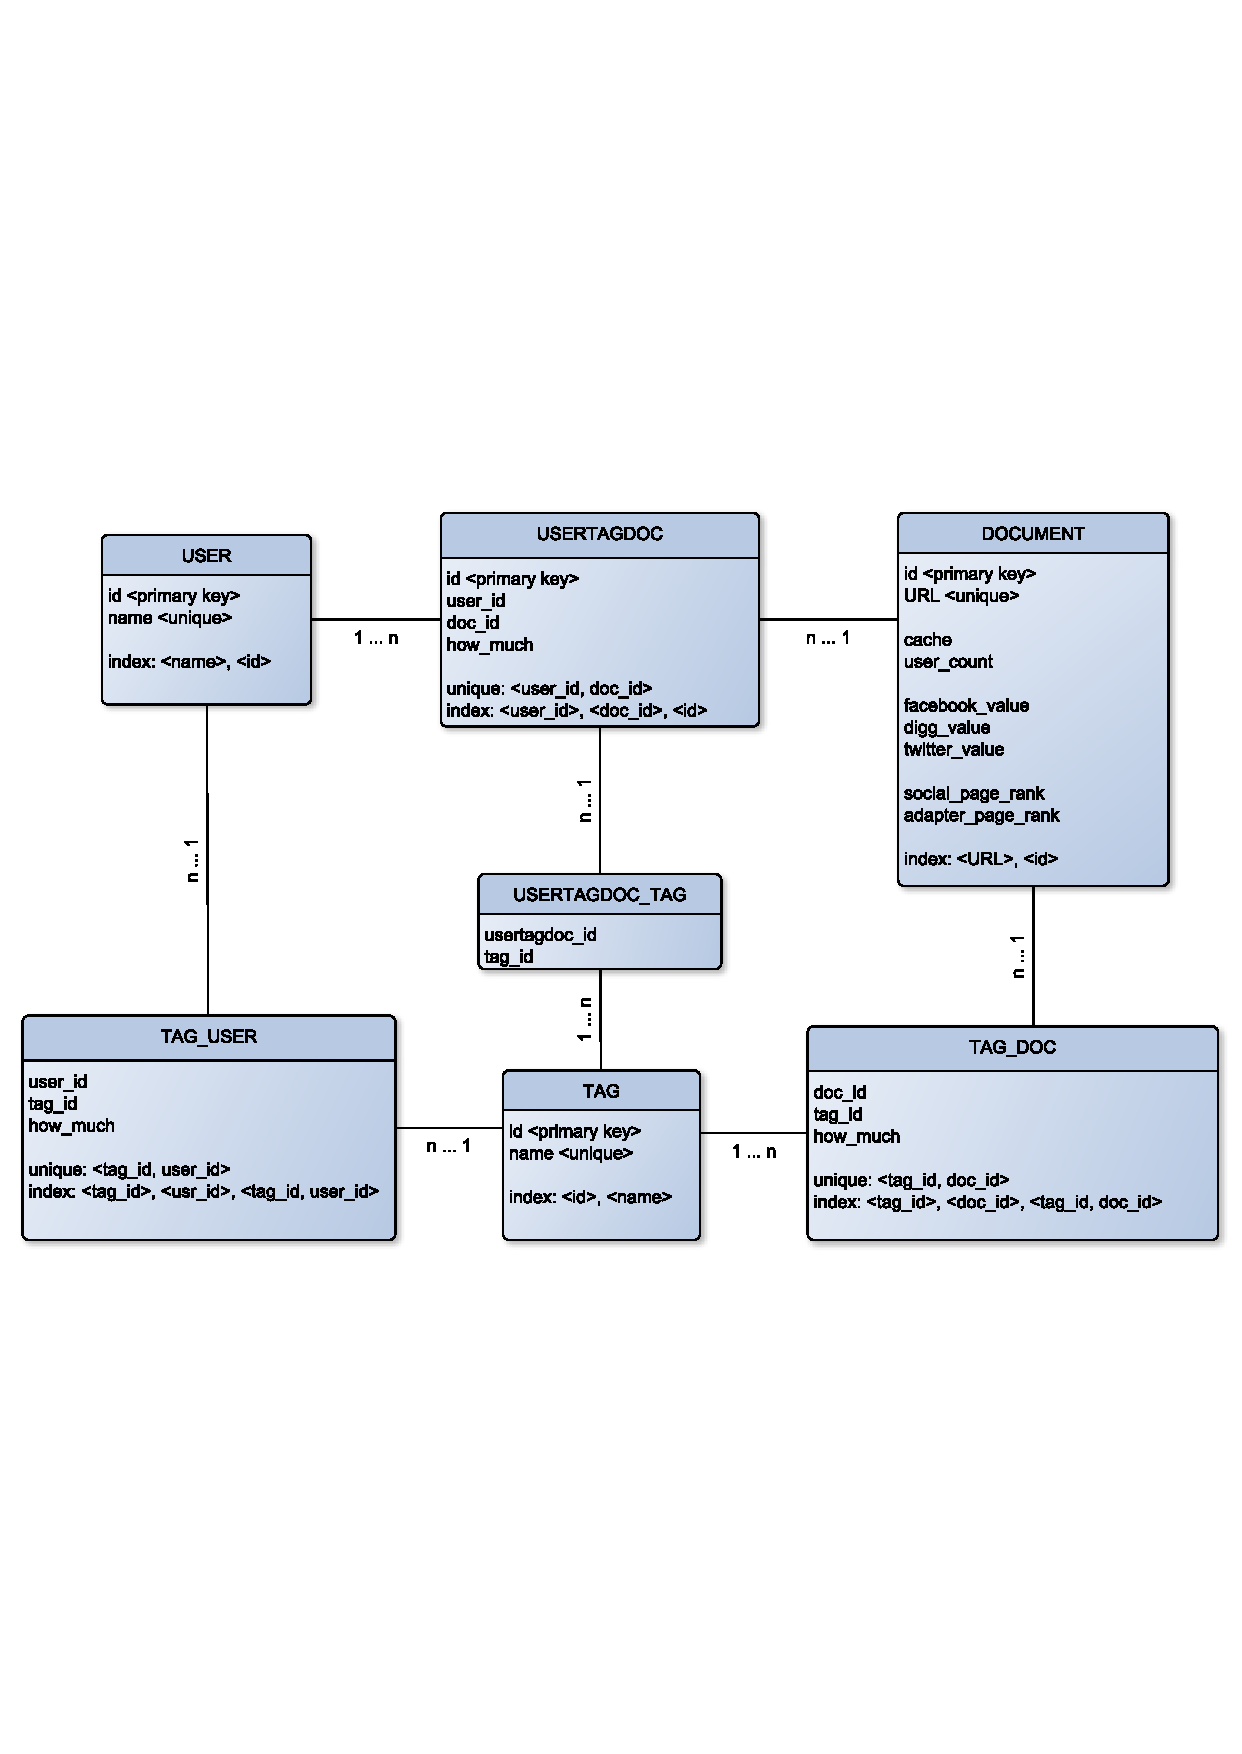
\includegraphics[width=1\textwidth]{database.pdf}
\caption{Schemat bazy danych}
\label{fig:db_fig}
\end{figure}

Baza danych składa się z trzech głównych tabel: User, Document i Tag. Zawierają one informację na temat użytkowników, dokumentów i adnotacji pobrane z serwisu delicous. W bazie danych znajdują sie też tabele: UserTagDoc i UserTagDoc\_tag, które służą do zapisania relacji między użytkownikami a dokumentami (usertagdoc) i adnotacjami (UserTagDoc\_tag). W tych tabelach zapisane są  informacje na temat tego czy dany użytkownik dodał dokument do serwisu i jakimi tagami została dana strona opisana.








\subsection{Tabele i pola pomocnicze}
Dodatkowo w bazie danych znajdują się dwie tabele: tag\_doc i tag\_user. Tabele tych zapisywane są dane wyliczone z pozostałych tabel. W tabeli tag\_doc znajdują się informację na temat tego ile razy przez różnych użytkowników dany dokument doc\_i  został dodany i opisany tagiem tag\_k. Odpowiednia w tabeli tag\_user znajdują się informację na temat ilości różnych dokumentów dodanych przez użytkownika usr\_n i opisanych tagiem tag\_m. Dane ilości różnych tagów którymi użytkownik usr\_l opisał dokument doc\_j przechowywane są w już istniejącej tabeli UserTagDoc.

Schemat bazy danych z zaznaczonymi nowymi tabelami i polem count w usertagdoc

W tabelach na różnych polach zostały dodane indeksy. Przyśpieszają one działanie aplikacji, pozwalają na szybsze operacja przy często używanych polach.
\subsection{Listing}
Poniżej znajduje się listing zapytania SQL tworzącego tabele w bazie danych.

\lstset{language=SQL}  
\begin{lstlisting}[frame=lines, caption={Skrypt tworzący tabele w bazie danych}, label={sql_all}] ]


CREATE TABLE `DOCUMENT` (
 `id` bigint(20) NOT NULL AUTO_INCREMENT,
 `url` varchar(255) NOT NULL,
 `digg_value` int(11) DEFAULT '0',
 `facebook_value` int(11) DEFAULT '0',
 `twitter_value` int(11) DEFAULT '0',
 `page_fetch` tinyint(1) DEFAULT '0',
 `tag_count` bigint(20) DEFAULT NULL,
 `user_count` bigint(20) DEFAULT NULL,
 `cache` text,
 `adapted_page_rank` double DEFAULT NULL,
 `social_page_rank` double DEFAULT NULL,
 PRIMARY KEY (`id`),
 UNIQUE KEY `url` (`url`)
) 

CREATE TABLE `TAG` (
 `id` bigint(20) NOT NULL AUTO_INCREMENT,
 `doc_count` bigint(20) DEFAULT NULL,
 `doc_dist_count` bigint(20) DEFAULT NULL,
 `tag` varchar(255) NOT NULL,
 `user_count` bigint(20) DEFAULT NULL,
 `adapted_page_rank` double DEFAULT NULL,
 PRIMARY KEY (`id`),
 UNIQUE KEY `tag` (`tag`)
)

CREATE TABLE `TAG_DOC` (
 `id` bigint(20) NOT NULL AUTO_INCREMENT,
 `doc_id` bigint(20) DEFAULT NULL,
 `tag_id` bigint(20) DEFAULT NULL,
 `how_much` int(11) DEFAULT '1',
 PRIMARY KEY (`id`),
 UNIQUE KEY `tag_doc` (`doc_id`,`tag_id`),
 KEY `doc_id` (`doc_id`,`tag_id`),
 KEY `tag_doc_doc` (`doc_id`),
 KEY `tag_doc_tag` (`tag_id`)
) 

CREATE TABLE `TAG_USR` (
 `id` bigint(20) NOT NULL AUTO_INCREMENT,
 `user_id` bigint(20) DEFAULT NULL,
 `tag_id` bigint(20) DEFAULT NULL,
 `how_much` int(11) DEFAULT '1',
 PRIMARY KEY (`id`),
 UNIQUE KEY `tag_user` (`user_id`,`tag_id`),
 KEY `user_id` (`user_id`,`tag_id`),
 KEY `tag_usr_doc` (`tag_id`),
 KEY `tag_usr_usr` (`user_id`)
)

CREATE TABLE `USER` (
 `id` bigint(20) NOT NULL AUTO_INCREMENT,
 `doc_count` bigint(20) DEFAULT NULL,
 `name` varchar(255) DEFAULT NULL,
 `new_data` tinyint(1) DEFAULT '1',
 `tag_count` bigint(20) DEFAULT NULL,
 `tag_dist_count` bigint(20) DEFAULT NULL,
 `adapted_page_rank` double DEFAULT NULL,
 PRIMARY KEY (`id`),
 UNIQUE KEY `name` (`name`)
)


CREATE TABLE `USERTAGDOC` (
 `id` bigint(20) NOT NULL AUTO_INCREMENT,
 `doc_id` bigint(20) DEFAULT NULL,
 `user_id` bigint(20) DEFAULT NULL,
 `how_much` int(11) DEFAULT NULL,
 PRIMARY KEY (`id`),
 UNIQUE KEY `user_id` (`user_id`,`doc_id`),
 KEY `FKB30EFAE96714BC07` (`doc_id`),
 KEY `FKB30EFAE9520DD4E4` (`user_id`),
 CONSTRAINT `FKB30EFAE9520DD4E4` FOREIGN KEY (`user_id`) REFERENCES
`user` (`id`),
 CONSTRAINT `FKB30EFAE96714BC07` FOREIGN KEY (`doc_id`) REFERENCES
`document` (`id`)
) 


CREATE TABLE `USERTAGDOC_TAG` (
 `USERTAGDOC_id` bigint(20) NOT NULL,
 `tags_id` bigint(20) NOT NULL,
 KEY `FK4C01D124CA702D03` (`tags_id`),
 KEY `FK4C01D1243D83CB28` (`USERTAGDOC_id`),
 CONSTRAINT `FK4C01D1243D83CB28` FOREIGN KEY (`USERTAGDOC_id`)
REFERENCES `usertagdoc` (`id`),
 CONSTRAINT `FK4C01D124CA702D03` FOREIGN KEY (`tags_id`) REFERENCES
`tag` (`id`)
) 

\end{lstlisting}

\end{document}

\section{Zbieranie danych}

	[TODO - OPIS CRAWLERÓW]

\subsection{Czyszczenie tagów przed zapisem}

Tagi pobierane z serwisu delicous nie zawsze są w postaci wymaganej przez aplikacje. Spowodowane to jest błędami użytkowników, czy też specyficznym stylem zapisywania tagów.

Niektóre tagi mają różne znaczenie w zależności od kontekstu, na przykład tag 'design' ma inne znaczenie w kontekście strony o programowaniu, a inne w kontekście strony o sztuce. Część użytkowników żeby poradzić sobie  z tym problemem dodają do tagów informacje mówiące o ich domenie. Często domena ma wygląd 'programming@design' czy 'art\#design'. 

Z powodu tego specyficznego zapisu każda etykieta, przed zapisaniem do bazy danych jest dzielona na 2 lub więcej słów w miejscach występowania popularnych znaków specjalnych. Dlatego też 

Dodane kontekstu do tagu mogłoby być przydatne w aplikacji, ale z powodu tego że każdy użytkownik ma swój specyficzny sposób opisywania dokumentów np: design@art i art\#design, trudno jest je zunifikować. Dodatkowym problemem jest to, że nie jest to sposób opisu używany przez wszystkich użytkowników. 


Adnotacje przypisywane przez użytkowników często kończą się lub zaczynają od znaków specjalnych. Jest to spowodowane np: błędami (dodatkowe przecinki) albo specyficznym stylem opisywania danych przez użytkownika. Wszystkie znaki specjalne z końca i początku dokumentu są usuwane przed dodaniem do bazy danych.

Przykłady danych przed i po ich oczyszczeniu:

\begin{itemize} 
    \item '@java' : 'java'
    \item '@@java' : 'java'
    \item  '\#java6@' : 'java6'
    \item  'design!\$\%@art' : 'design', 'art'
    \item  'art!\#,': 'art'
\end{itemize}







\section{Implementacja algorytmów Social PageRank i Adapted PageRank}

Zarówno algorytm Social PageRank i Adapted PageRank wykorzystują w trakcie każdej iteracji szcześć macierzy. Sa to macierze opisane poniżej i ich traspozycje:

\begin{itemize}
\item $M_{DU}$: macierz $N_D \times N_D$ asocjacyjna między dokumentami a użytkownikami, która w każdej komórce $M_{DU}(d_m, u_k)$ zawiera ilość tagów, którymi dany użytkownik $u_k$ opisał wybrany dokument $d_m$.
\item $M_{UT}$: macierz $N_U \times N_T$  asocjacyjna między użytkownikami a tagami, zawerająca w komórce ilość dokumentów opisanych wybranym tagiem przez danego użytkownika
\item $M_{TD}$: macierz $N_T \times N_D$ asocjacyjna między tagami a dokumentami, zawierająca w komórach liczbę użytkowników, którzy dany dokument opisali wybranym tagiem.

\end{itemize}

Algorytmy te działały na około danych składających sie z około 1,000,000 użytkowników, 600,000 dokumentów i 80,000 tagów. Macierze utworzone z tych danych są duże. Dodatkowo, w algorytmie Adapted PageRank używamy macierzy, która jest stworzona ze wszystkich 6-ciu opisanych powyżej:

\[
 G_f =
 \begin{pmatrix}
  0                     & M_{DU}       & M_{TD}^T \\
  M_{DU}^T  & 0                     & M_{UT}     \\
  M_{TD}       & M_{UT}^T   & 0 
 \end{pmatrix}
\]

Problemem jest nie tylko sama wielkośc macierzy, które nie mogą zmieścić sie jednocześnie w pamięci, ale również ich zawartość. Wyliczanie danych przy każdej iteracji jest bardzo czasochłonne. Dlatego, żeby nie wyliczać zawartości macierzy przy każdej iteracji, potrzebujemy zapamiętać ich zawartość. Dodatkowo, wyliczanie choćby jednarozowe danych, jest bardzo kosztowne.

Żeby rozwiązać te problemy, napoczątku wykonywany jest preprocessing w bazie danych, wyliczający wymagane dane. Następnie, dane te są zapisywane na dysku w łatwą do użycia później strukturę danych, która zawiera tylko określoną ilość wierszy macierzy.


Pliki te później są używane jako fragmenty macierzy. Na tych fragmentach wykonywane są wymagane obliczenia. Kolejne wyniki obliczeń są następnie łączone i przekazywane do kolejnej iteracji, albo zwracane jako wynik algorytmu.







%\usepackage{algorithmic}
%\usepackage{algorithm}
%\usepackage{program}
%\usepackage{programs}



\section{Preprocessing w bazie danych}

W bazie danych wyliczone zostają informacje potrzebne do późniejszego utworzenia macierzy używanych w algorytmach Adapted PageRank i Social PageRank. Algorytmy te przy każdym przebiegu korzystają z tych samych macierzy, obliczanie ich przy każdej iteracji wymagałoby zbyt dużego nakładu czasu. Dane te są wyliczane w dwóch częściach. Na początku wyliczane są w bazie danych i zapisywane w pomocniczych tabelach. Następnie zapisywane są one do do struktury i serializowane w oddzielnych plikach. Pliki te są później używane do tworzenia macierzy.

Informacje te zostaną zapisane w tabeli USERTAGDOC w polu how\_much i w tabelach TAG\_USR i TAG\_DOC. Wyliczenie tych informacji pozwoli później na szybszy dostęp do nich.

Czas wykonania preprocessingu w bazie danych jest różny. Jak widać w tabeli poniżej (\ref{tab:czas_tabele}) najwięcej czasu trwało tworzenie tabeli TAG\_USR i powstało w niej najwięcej nowych rekordów. Wykonywanie tych obliczeń przy każdej iteracji algorytmu spowodowałoby znacznie zwiększenie czasu działania aplikacji.

\begin{table}[hbp]
  \centering
    \begin{tabular}{ | c | p{3cm}| p{3cm} | }
    \hline
    Tabela & czas wykonania polecenia & ilość powstałych rekordów  \\ 
    \hline
    TAG\_USR & FIXME & FIXME   \\ 
    \hline
    TAG\_DOC & ok 3h &  FIXME  \\ 
    \hline
    USERTAGDOC & FIXME  & FIXME  \\ 
    \hline
    \end{tabular}
     \caption{Czas wykonania wypełnienia odpowiednich tabel w bazie danych !FIXME!}
    \label{tab:czas_tabele}
   
\end{table}


Poniżej znajdują się listingi zapytań SQL obliczających pola tabeli USERTAGDOC \ref{sql_usrtagdoc} i wypełniające tabele TAG\_USR (\ref{sql_tag_doc}) i TAG\_DOC (\ref{sql_tag_usr}). 


\lstset{language=SQL}   
\begin{lstlisting}[frame=lines, caption={Skrypt dodający dane do tabeli tag\_doc}, label={sql_tag_doc}]
insert into tag_doc (doc_id, tag_id, how_much) 
select d.new_id, tag.new_id, count(utd.user_id)
from 
tag, 
usertagdoc_tag as utd_t,
usertagdoc as utd, document as d
where
d.id = utd.doc_id 
and utd_t.usertagdoc_id = utd.id 
and utd_t.tags_id = tag.id
group by utd.doc_id, tag.id;

\end{lstlisting}

\begin{lstlisting}[frame=lines, caption={Skrypt dodający dane do tabeli tag\_usr}, label={sql_tag_usr}]]
insert into tag_usr (tag_id, user_id, how_much)
select utd.user_id, tag.new_id, count(utd.doc_id)
from
tag,
usertagdoc_tag as utd_t,
usertagdoc as utd
where
utd_t.usertagdoc_id = utd.id and
utd_t.tags_id = tag.id
\end{lstlisting}

\begin{lstlisting}[frame=lines, caption={Skrypt updatujący pole how\_much w tabeli usertagdoc}, label={sql_usrtagdoc}] ]
update usertagdoc utd
set how_much = (select count(distinct tags.tags_id)
from usertagdoc_tag tags
where utd.id = tags.usertagdoc_id);
\end{lstlisting}


\subsection{Preprocessing: zapis do plików}
Po wyliczeniu w bazie danych pomocniczych tabel, wyniki są pobierane przez program, a następnie zapisywane do pliku. Ponieważ pamięć maszyny ogranicza wielkość macierzy na której jesteśmy w stanie operować, tworzone pliki zawierają tylko wyznaczoną ilość wierszy. Ilość wierszy macierzy zapisanych w pliku jest konfigurowalna i zależna od przydzielonej pamięci aplikacji.


W czasie działania algorytmów wymagane są również traspozycje wybranych macierzy. Ponieważ ograniczenia pamięciowe uniemożliwiają obrócenie macierzy w pamięci, w plikach zapisane zostaną również traspozycje macierzy.


\begin{figure}[htb]
\centering
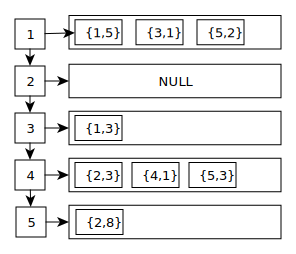
\includegraphics[width=0.5\textwidth, trim = 0mm 33mm 0mm 33mm, clip]{file_processing.pdf}
\caption{Struktura zapisana w pliku}
\label{fig:preprocessing_fig}
\end{figure}

Wynikiem działania tej części preprocesingu jest struktura będąca HashMapą. Zawierająca ona w komórce $i$ listę wszystkich niezerowych elementów znajdujących się w i-tym wierszu macierzy wraz z ich wartościami. Figura \ref{fig:preprocessing_fig} pokazuje fragment macierzy, który zostanie zapisany do pliku. Poniżej znajduje sie macierz $M_{5,5}$, która powstanie ze struktury przedstawionej na \ref{fig:preprocessing_fig}


\[
 M_{5,5} =
 \begin{pmatrix}
5 & 0 & 1 & 0 & 2\\
0 & 0 & 0 & 0 & 0\\
3 & 0 & 0 & 0 & 0\\
0 & 3 & 0 & 1 & 3\\
0 & 8 & 0 & 0 & 0\\

 \end{pmatrix}
\]


\subsection{Inne metody przyśpieszenia wykonywanych preprocesingów}

Jednym z głównym problemów jest to, że w czasie wykonywania wymienionych powyżej procedur, tabele USER, TAG i DOCUMENT są zablokowane na zmiany. W działającej aplikacji byłoby to poważnym problemem.  

Można poradzić sobie z tym problemem poprzez posiadanie kopi bazy danych i uzupełnianie obydwu jednocześnie. Dzięki czemu operacje wymagające dużej ilości czasu, mogłyby być wykonane na innej bazie. Po dokonaniu wszystkich obliczeń wymagane jest zsynchronizowanie obydwu baz danych.

Inną możliwością jest zrównoleglenie wykonywanych obliczeń. Możliwe jest na przykład: podzielenie obliczenia tabel TAG\_DOC, TAG\_USER i USERTAGDOC na różne maszyny. Dodatkową możliwością jest podzielenie samych tabel na różne procesy. Na przykład wyliczanie tabeli TAG\_DOC można podzielić na niezależne procesy ze względu na pole ID obiektów z tabeli TAG. Analogicznie można przeprowadzić taki podział dla innych tabel.

Kolejną możliwością są zmiany danych w tabelach TAG\_DOC, TAG\_USER i USERTAGDOC w czasie kiedy dodawane są nowe rekordy do tabel USER, DOCUMENT i TAG. Wyeliminowało by to potrzebę wykonywania opisane powyżej preprocesingu, ale stanowiło by problem przy tworzeniu macierzy. Tworzenie macierzy (dokładnie: plików z których następnie tworzona jest macierz) jest czasochłonne i wymaga zatrzymania zmian dokonywanych na tabelach TAG\_DOC, TAG\_USER i USERTAGDOC. Problem ten dałoby się rozwiązać przez np: posiadanie kopi wymienionych wcześniej tabel. Synchronizacja kopi tabeli i głównej tabeli nie zajmowała by aż tak wiele czasu. Pomysł ten spowodował by jeszcze jeden potencjalnie groźny problem. Ilość operacji, które trzeba by wykonać w czasie gdy dodawane są nowe rekordy do tabel, znacznie by się zwiększyła. Mogłoby to spowodować większą awaryjność np: problemy z transakcjami.













\documentclass[11pt,a4paper]{report}

\usepackage[polish]{babel}
\usepackage[utf8x]{inputenc}
\usepackage{polski}
%\usepackage[T1]{fontenc}
\frenchspacing
\usepackage{indentfirst}
\usepackage{amsthm}
\usepackage{amsmath}
\usepackage{algorithmic}
\usepackage{algorithm}
\usepackage{program}
\usepackage{programs}
\usepackage{array}
\usepackage{multirow}
\usepackage{graphicx}
\usepackage{listings}
\usepackage{listing}
\usepackage{float}
\pagenumbering{arabic}

\graphicspath{{img/}}

\begin{document}
\tableofcontents
\chapter{Macierze}
\section{Tworzenie macierzy na potrzeby algorytmów}
W algorytmach potrzebne są głównie 3 rodzaje macierzy i ich transpozycje. Macierze te są tworzone z danych zebranych z serwisu delicous:
\begin{itemize}
	\item $M_{UT}$ macierz ta zawiera w komórce $m_{n,m}$ informacje o ilości dokumentów dodanych przez użytkownika $u_n$ i opisanych tagiem $t_m$. Dane, z których zostaje utworzona ta macierz znajdują się w tabeli TAG\_USR. Tabela ta została wyliczona w czasie preprocessingu.
	\item $M_{TD}$ macierz ta zawiera w komórce $m_{n,m}$ informacje o ilości użytkowników którzy opisali tagiem $t_n$ dokument $d_m$. Źródłem danych dla taj macierzy jest tabela TAG\_DOC
	\item $M_{DU}$ analogicznie, ta macierz zawiera dane na temat ilości tagów. Informacje pobierane są z tabeli USERTAGDOC
\end{itemize}

Wykorzystywane są one w kolejnych iteracjach algorytmu Social PageRank. Przy algorytmie Adapted PageRank również są one używane pośrednio. Struktura na której operuje algorytm Adapted pagerank jest macierzą złozoną z macierzy $M_{UD} , M_{TD}, M_{UT}$ i ich transpozycji. Macierzy używana w algorytmie wygląda następująco:

\[
 G_f =
 \begin{pmatrix}
  0                     & M_{DU}       & M_{TD}^T \\
  M_{DU}^T  & 0                     & M_{UT}     \\
  M_{TD}       & M_{UT}^T   & 0 
 \end{pmatrix}
\]

Ważną cechą macierzy na których przeprowadzane są operacje jest to, że są to macierze rzadkie. Liczba niezerowych komórek w macierzy wynosi: 

\section{Operacje przeprowadzane na macierzach}
W każdej iteracji algorytów główna operacją przeprowadzaną jest mnożenie wymienionych wcześniej macierzy przez wektor. Operacja ta jest przeprowadzana do czasu uzyskania zbieżności wartości wektora wynikowego.

Z powodu wielkości macierzy w aplikacji nie możemy wczytać bezpośrednio całych macierzy do pamięci i na nich operować. Dodatkowo używana biblioteka stawia ograniczenie na iloczyn kolumn i wierszy takie że: $ilosc\_kolumn * ilosc\_wierszy <= 2^{31}-1$.  Gdzie wartość $2^{31}-1$ jest to maksymalna liczba jaką można przypisać zmiennej typu integer w języku Java. 



\subsection*{Implementacja}

\begin{figure}[htb]
\centering
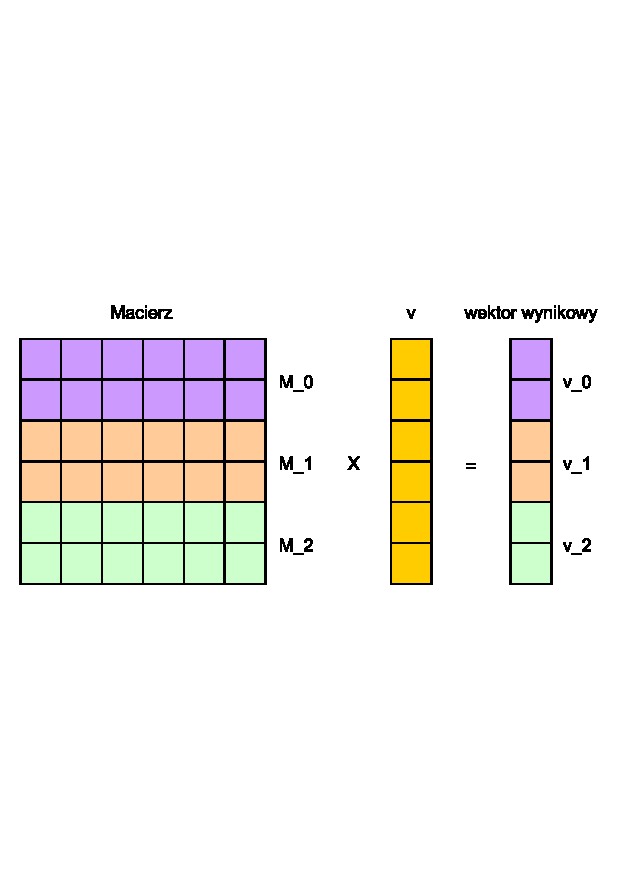
\includegraphics[width=1\textwidth, trim = 0mm 45mm 0mm 50mm, clip]{matrix_multiply.pdf}
\caption{Mnożenie macierzy przez wektor v}
\label{fig:matrix_mult_fig}
\end{figure}

Mnożenie macierzy odbywa się częściami. Bierzemy fragment macierzy: $M_{n}$ i mnożymy go przez wektor $v$. Wynikiem jest wektor $p_n$, który stanowi n-ty fragment wynikowego wektora. Powstałe fragmenty wektora łączymy razem, w odpowiedniej kolejności otrzymując w ten sposób w wektor wynikowy (\ref{fig:matrix_mult_fig})




\lstset{language=Python}
\begin{lstlisting}[frame=lines, caption={Mnożenie macierzy przez wektor v}, label={list:matrix_mult_fig}] ]
def matrix_multiply(v, matrix_source):
	v_return = empty_vector()  #wektor zwracany
	for matrix_part in matrix_source.get_part_matrixes():
		#mnozenie macierzy i wektora
		v_part = multiply(matrix_part, v) 
		# dokladamy wyliczony fragment wektora na koniec
		v_return.append(v_part)   
	return v_return 
\end{lstlisting}

Mnożenie odbywa się poprzez funkcje z biblioteki Colt. Biblioteka ta uwzględnia to, że macierz na której odbywają się operacje jest macierzą rzadką. Oszczędzana jest pamięć przez zapisywanie tylko niezerowych elementów. W czasie mnożenia przez wektor pomijane są wszystkie zerowe komórki, przez co sama operacja mnożenia jest krótka. Najwięcej czasu zajmuje samo tworzenie częściowych  macierzy i ładowanie plików zawierających kolejne fragmenty macierzy. 


\subsection{Metody przyśpieszenia obliczeń}

Opisana powyżej metoda nie mogłaby zostać wykorzystana w działającej z klientem aplikacji. Przy tylko 1 milionie dokumentów czas wykonania algorytmu Social PageRank wynosi około 36 godzin. Poniżej opisanych jest kilka możliwych pomysłów na ulepszenie i przyśpieszenie działania aplikacji

\begin{itemize}
	\item Sam wybór języka programowania, w którym została wykonana aplikacja nie jest najlepszym wyborem. Maszyna wirtualna Javy nie jest bardzo wydajna jeśli chodzi o szybkość obliczeń, dodatkowo dochodzą ograniczenia związane np: z pamięcią. Jedną z możliwości jest przepisanie całej aplikacji na inny język. Możliwe jest również przepisanie tylko fragmentów a następnie ich uruchamianie z aplikacji. 
	\item Proste zrównoleglenie obliczeń: wykorzystując metodę dzielenia macierzy na kawałki, możliwe jest podzielenie macierzy na różne procesory/maszyny. Każdy proces po zakończeniu obliczania swojej części zapisałby wynikowy wektor do np: bazy danych, w której następowałaby synchronizacja procesów. 
	\item Obliczanie przy użyciu GPU/CUDA: możliwe jest wykorzystanie GPU do wykonania obliczeń na macierzach. Obecne jednostki graficzne  ( naprzykład: GF100 o nazwie kodowej "Fermi") zawierają dodatkowe technologie wspomagające operacje na macierzach rzadkich. 
	\item Obliczanie kolejnych iteracji mogłoby również być przerzucone na zewnętrzną aplikacji np: MATLAB.
\end{itemize}

\end{document}
\chapter{Dane [TODO]}

[ statystyki danych, czyszczenie danych, wyszukiwanie outlierów, ... ]


\section{Testy}
\subsection{Opisy przeprowadzonych eksperymentów}

Dane testowe składają się ze zbioru prac naukowych pobranych ze stron Arxiv i PMC. Każdy dokument posiada przypisane mu tagi i ilość cytowań w innych pracach naukowych. 



\subsection{Jakość wyszukiwania}

Każdemu dokumentowi została przypisana jego 'jakość'. Jakość dokumentu została określona jako znormalizowana ilości cytowań danego dokumentu w innych pracach naukowych. Należy tutaj zaznaczyć, że przy dodawaniu danych testowych do bazy danych, liczba użytkowników, którzy dodali dany dokument, jest równa ilości cytowań. Może to mieć wpływ na wyniki testów. Jednakże przy obydwu algorytmach, wpływ maja nie tylko użytkownicy, ale również tagi i ich jakość. Dodatkowo, przy tworzeniu macierzy, liczba ta nie jest używana bezpośrednio.



\begin{figure}[tb]
    \centering
    \includegraphics[width=\linewidth]{test_jakosc_genome.png}
    \caption{Wyniki testów pod względem jakości, wyszukiwanie słowa: 'genome'}
    \label{fig:jakosc-genome}

\end{figure}

\begin{figure}[tb]
    \centering
    \includegraphics[width=\linewidth]{test_jakosc_hashimoto.png}
    \caption{Wyniki testów pod względem jakości, wyszukiwanie słowa: 'hashimoto'}
    \label{fig:jakosc-hashimoto}

\end{figure}

\begin{figure}[tb]
    \centering
    \includegraphics[width=\linewidth]{test_jakosc_immunodeficiency.png}
    \caption{Wyniki testów pod względem jakości, wyszukiwanie słowa: 'immunodeficiency'}
    \label{fig:jakosc-immunodeficiency}

\end{figure}

\begin{figure}[tb]
    \centering
    \includegraphics[width=\linewidth]{test_jakosc_pathogen.png}
    \caption{Wyniki testów pod względem jakości, wyszukiwanie słowa: 'pathogen'}
    \label{fig:jakosc-pathogen}

\end{figure}

\begin{figure}[tb]
    \centering
    \includegraphics[width=\linewidth]{test_jakosc_retrovirus.png}
    \caption{Wyniki testów pod względem jakości, wyszukiwanie słowa: 'retrovirus'}
    \label{fig:jakosc-retrovirus}

\end{figure}


Miarą testów jest znormalizowany zysk całościowy (ang. Normalized Discounted Cumulative Gain). Wyliczany jest on według wzoru:

\begin{equation}
   nDCG_{p} = \frac{DCG_{p}}{IDCG_{p}} 
\end{equation}

Gdzie DCG to zysk całościowy (ang. Discounted Cumulative Gain), a IDCG to idealny zysk całościowy obliczony jako maksymalny możliwy wynik dla danego zapytania $p$ .

Zysk całościowy wyliczany jest za pomocą wzoru:

\begin{equation}
    DCG_{p} = rel_{1} + \sum_{i=2}^{p} \frac{rel_{i}}{\log_{2}(i+1)} 
\end{equation}

Gdzie $rel_i$ jest jakością dokumentu otrzymanego w wyniku na pozycji $i$.

Testy zostały przeprowadzone na zbiorze wszystkich zebranych dokumentów. Do wyników brane były tylko dokumenty ze zbioru prac naukowych. W przypadku uzyskania w wyniku dokumentu z poza tego zbioru, jakość tego wyniku równa jest zero. Dla porównania przedstawiono również wyniki testów, w których pominięto wyniki z poza zbioru.

Można zauważyć na wykresach, że otrzymujemy lepsze wyniki przy użyciu algorytmu SocialPageRank w zbiorze danych z których usunięto elementy zerowe. Dokumenty otrzymane przy pomocy innych metod są gorszej jakości. 

W zbiorze w którym występowały dokumenty o jakości zero, Lucene i AdaptedPageRank dawały zdecydowanie lepsze wyniki. Mimo, że koszt całościowy jest niski, to w przypadku algorytmu SocialPageRank jest on w większości zerowy. Nawet jeśli jakość tych wyników jest niska, AdaptedPageRank i Lucene dają poprawne wyniki w pierwszych 10 elementach.

Zaobserwować również wysokie wyniki otrzymane przy pomocy Lucene. W tym przypadku, może to byś spowodowane wysoką jakością publikacji naukowych w porównaniu do treści stron internetowych.





\subsection{Precyzja wyszukiwania}



\begin{figure}[tb]
    \centering
    \includegraphics[width=0.9\linewidth]{test_wyniki_prec_genome.png}
    \caption{Wyniki precyzji wyników, wyszukiwanie słowa: 'Genome', }
    \label{fig:prec-genome}

\end{figure}



\begin{figure}[tb]
    \centering
    \includegraphics[width=0.9\linewidth]{test_wyniki_prec_geophisics.png}
    \caption{Wyniki precyzji wyników, wyszukiwanie słowa: 'Geophisics', }
    \label{fig:prec-geophisics}

\end{figure}

\begin{figure}[tb]
    \centering
    \includegraphics[width=0.9\linewidth]{test_wyniki_prec_hashimoto.png}
    \caption{Wyniki precyzji wyników, wyszukiwanie słowa: 'Hashimoto', }
    \label{fig:prec-hashimoto}

\end{figure}


\begin{figure}[tb]
    \centering
    \includegraphics[width=0.9\linewidth]{test_wyniki_prec_immunodeficiency.png}
    \caption{Wyniki precyzji wyników, wyszukiwanie słowa: 'Immunodeficiency', }
    \label{fig:prec-immunodeficiency}

\end{figure}


\begin{figure}[tb]
    \centering
    \includegraphics[width=0.9\linewidth]{test_wyniki_prec_retrovirus.png}
    \caption{Wyniki precyzji wyników, wyszukiwanie słowa: 'Retrovirus', }
    \label{fig:prec-retrovirus}

\end{figure}



Kolejną miarą wyników algorytmów jest precyzja. Miara ta będzie sprawdzana dla pierwszych  $n$ wyników:

\begin{equation}
Prec(n) = \frac{number\_rel_n}{n}
\end{equation}

Precyzja dla $n$ jest to ilość poprawnie wybranych elementów ($number\_rel$) dla pierwszych $n$ elementów.


Dla posiadanych danych, precyzja odpowiedzi została przetestowana dla pierwszych 20 wyników. Przykładowe wyniki znajdują się na wykresach \ref{fig:prec-genome},  \ref{fig:prec-geophisics},  \ref{fig:prec-hashimoto},  \ref{fig:prec-immunodeficiency} i  \ref{fig:prec-retrovirus}.



Można zaobserwować, że poza wykresem \ref{fig:prec-retrovirus} i \ref{fig:prec-geophisics} (od elementu 15) najlepsze wyniki uzyskujemy używając algorytmu Adapted PageRank. Przy użyciu Lucene otrzymujemy gorsze wyniki, ale ciągle dość wysokie. Algorytm SocialPageRank w pierwszych 20 wynikach podaje bardzo złe wyniki, często zerowe.



\subsection{Średni wzajemny ranking}


Przeprowadzone zostały również testy biorące pod uwagę cały zbiór
dokumentów, czyli dokumenty zebrane z serwisu delicious.com i dokumenty złożone
z publikacji naukowych. Problemem w testowaniu algorytmów wyszukiwania na
takim dużym zbiorze jest sam proces ocenienia otrzymanych odpowiedzi.  Dodatkowo
należy sprawdzić czy w zbiorze pominiętych dokumentów nie znajdują się
wyniki, które mogą nas interesować. Dlatego też do przeprowadzenia
tych testów użyto miary 'średniego wzajemnego rankingu', która bierze
pod uwagę tylko wybrany zbiór zapytań i jedną szukaną odpowiedz.


Średni wzajemny ranking (MMR, Mean reciprocal rank) jest miarą pozwalającą
na ocenianie jakości wyników zwracanych jako lista elementów
posortowanych według trafności. Kryterium to bierze pod uwagę zbiór
zapytań i jedna poprawna odpowiedz. Mierzona jest pozycja, na której
znajduję się interesująca nas odpowiedz. Dla przykładu, jeśli w
zbiorze zapytań znajduję się fraza 'bbc' oczekujemy, że główna strona
internetowa serwisu informacyjnego BBC będzie na wysokiej pozycji w
rankingu. Im dalej w wynikach znajduje się oczekiwana odpowiedz, tym
gorszy będzie wynik MMR.

Średni wzajemny ranking (MMR) wyrażany jest wzorem:

\begin{equation}
    \text{MRR} = \frac{1}{|Q|} \sum_{i=1}^{|Q|} \frac{1}{\text{rank}_i}
\end{equation}
Gdzie:
\begin{itemize}
\item $Q$ - zbiór zapytań,
\item $rank_i$ - pozycja poprawnego wyniku.
\end{itemize}


Do testów wybrane zostało wybrane dziesięć stron internetowych i zapytania
opisujące je w jednoznaczny sposób. Ponieważ nie zawsze główne strony znajdują się w bazie danych, jako wynik wystarczający uznawana jest również strona będącą w tej samej domenie. Dla przykładu, dla zapytania 'BBC' akceptowane są strony bbc.co.uk i bbc.co.uk/tv jako poprawne odpowiedzi.

 W tabeli \ref{tab:mmr} znajduje się zbiór zapytań i numer pozycji w wynikach, na której otrzymaliśmy poszukiwaną stronę. Wynik zero oznacza brak oczekiwanego wyniku w pierwszych dwudziestu odpowiedziach.

\begin{table}[htb]
  \centering
    \begin{tabular}{ | l | l | l | l | l | }
\hline
  Zapytanie  & Lucene & SocialPageRank & AdaptedPageRank & Inne serwisy \\
\hline
Debian & 7  &  4  & 0  & 0\\
BBC &   2 &  0  & 2  &  5 \\
Intel & 1  & 8  & 0  & 0 \\
Deviantart & 1  & 2  & 0 &  6\\
Pastebin & 1 &  0  & 8 &  3\\
Wikipedia & 4 &  1  & 1 &  14\\
Guardian & 2 &  4  & 1 &  6\\
Youtube & 0  & 0  & 2  & 11 \\
Sourceforge & 3 & 3  & 3 &  2 \\
\hline
\end{tabular}
  \caption{ Pozycja odpowiedzi w wynikach w zależności od algorytmu i zapytania}
  \label{tab:mmr}
\end{table}



Wyniki zostały również przedstawione w postaci figury \ref{fig:wyniki-mmr}. Tak samo jak w pojedynczych winkach jak uśrednionych można zaobserwować, że najlepsze wyniki otrzymujemy przy użyciu frameworku Lucene, czyli algorytmu TF-IDF. 



\begin{figure}[h]
    \centering
    \includegraphics[width=0.9\linewidth]{mmr.png}
    \caption{Średni wzajemny ranking }
    \label{fig:wyniki-mmr}

\end{figure}

















\bibliographystyle{plain}
\bibliography{biblio}


\end{document}
